
\documentclass[compress]{beamer}

%\usepackage{beamerthemesplit}
\usepackage{xmpmulti}

\usepackage{booktabs}
\usepackage{graphicx,float,wrapfig, bbm}
\usepackage{amsfonts, bbold, comment}
\usepackage{mdwlist}
\usepackage{subfigure}
\usepackage{colortbl}
\usepackage{overpic}
\usepackage{pdfpages}
\usepackage[normalem]{ulem}
\usepackage{multirow}

\pgfdeclareimage[width=\paperwidth]{mybackground}{../../common/boulder.pdf}

\newcommand{\slda}[0]{\abr{slda}}
\newcommand{\bm}[1]{\mbox{\boldmath$#1$}}
\newcommand{\lda}[0]{\abr{lda}}
\newcommand{\explain}[2]{\underbrace{#2}_{\mbox{\footnotesize{#1}}}}
\newcommand{\itmspace}[0]{\hspace{2cm}}
\newcommand{\pos}[1]{{\texttt{#1}}}
\newcommand{\e}[2]{\mathbb{E}_{#1}\left[ #2 \right] }
\newcommand{\ind}[1]{\mathbb{I}\left[ #1 \right] }
\newcommand{\abr}[1]{\textsc{#1} }
\newcommand{\ex}[1]{\mbox{exp}\left\{ #1\right\} }
\newcommand{\g}{\, | \,}
\newcommand{\citename}[1]{#1 }
\newcommand{\fsi}[2]{
\begin{frame}[plain]
\vspace*{-1pt}
\makebox[\linewidth]{\includegraphics[width=\paperwidth]{#1}}
\begin{center}
#2
\end{center}
\end{frame}
}


\newcommand{\danquote}[1]{

\begin{flushright}
\begin{overpic}[width=5.5cm,tics=10]{general_figures/speech_bubble}
	\put(10,30) { \parbox{4cm}{#1 }}
\end{overpic}

\includegraphics[width=1.5cm]{general_figures/milkman_dan}
\end{flushright}
}


\newcommand{\gfxt}[2]{
\begin{center}
	\includegraphics[width=#2\linewidth]{reading_tea_leaves/#1}
\end{center}
}

\newcommand{\gfxi}[2]{
\begin{center}
	\includegraphics[width=#2\linewidth]{interpretability/#1}
\end{center}
}

\newcommand{\gfxs}[2]{
\begin{center}
	\includegraphics[width=#2\linewidth]{simtrans/#1}
\end{center}
}

\newcommand{\gfxq}[2]{
\begin{center}
	\includegraphics[width=#2\linewidth]{qb/#1}
\end{center}
}


\newif\ifjobtalk\jobtalktrue
\newif\iflong\longtrue

\usetheme[
          showdate=true,                     % show the date on the title page
          alternativetitlepage=true,         % Use the fancy title page.
          titlepagelogo=general_figures/shell,              % Logo for the fir\
st page.
          ]{UMD}


\title[]{If You Want Interpretable AI, Measure It}
\author{ Jordan Boyd-Graber}
\date{2023}

\institute[] % (optional, but mostly needed)
{University of Maryland}


%gets rid of bottom navigation symbols
\setbeamertemplate{navigation symbols}{}

%gets rid of footer
%will override 'frame number' instruction above
%comment out to revert to previous/default definitions
\setbeamertemplate{footline}{}

\begin{document}

\frame{
\titlepage
\tiny
}

\begin{frame}[plain]
\vspace*{-1pt}
\only<1>{\makebox[\linewidth]{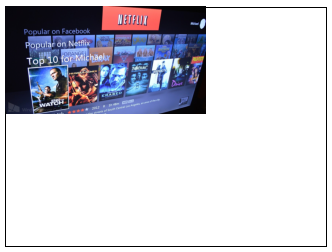
\includegraphics[width=\paperwidth]{general_figures/ml_intro_1}}}
\only<2>{\makebox[\linewidth]{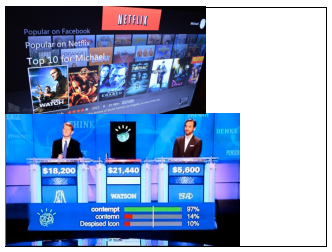
\includegraphics[width=\paperwidth]{general_figures/ml_intro_2}}}
\only<3>{\makebox[\linewidth]{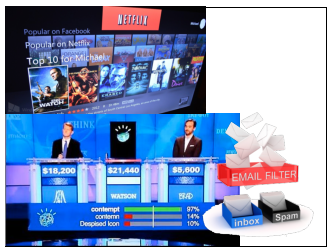
\includegraphics[width=\paperwidth]{general_figures/ml_intro_3}}}
\only<4>{\makebox[\linewidth]{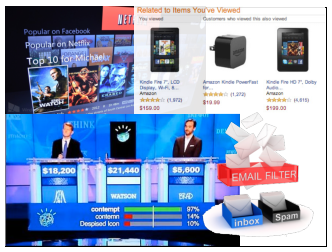
\includegraphics[width=\paperwidth]{general_figures/ml_intro_4}}}
\only<5>{\makebox[\linewidth]{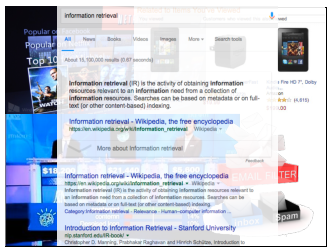
\includegraphics[width=\paperwidth]{general_figures/ml_intro_5}}}
\only<6->{\makebox[\linewidth]{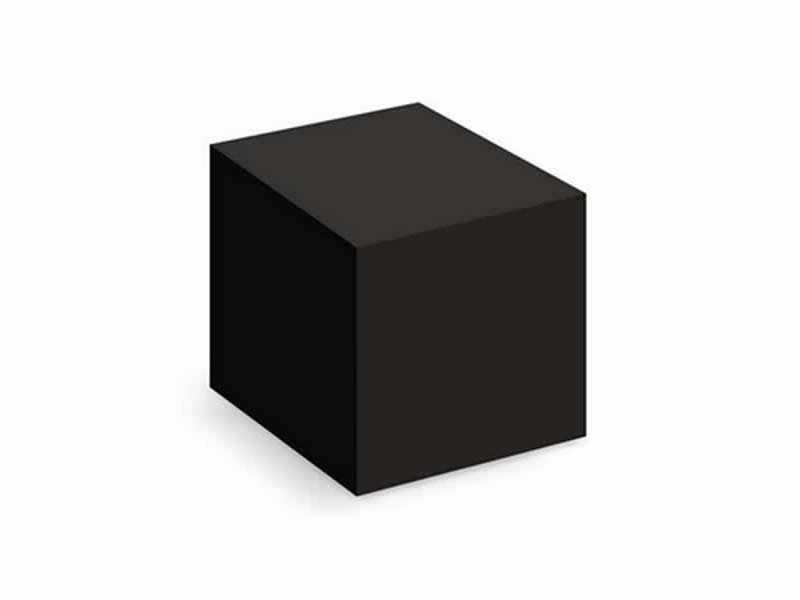
\includegraphics[width=\paperwidth]{general_figures/blackbox}}}
\only<7>{

\vspace{-5cm}
\begin{block}{Outline}
  \begin{itemize}
  \item AI should be interpretable
    \item We should measure interpretability    
  \item Proposal for Unsupervised Methods (Topic Models)
    \item Proposal for Supervised Methods \\ (Question Answering / Translation)
  \end{itemize}
\end{block}

}
\end{frame}


\begin{frame}{Interpretability/Human-Centered AI is Big!}
  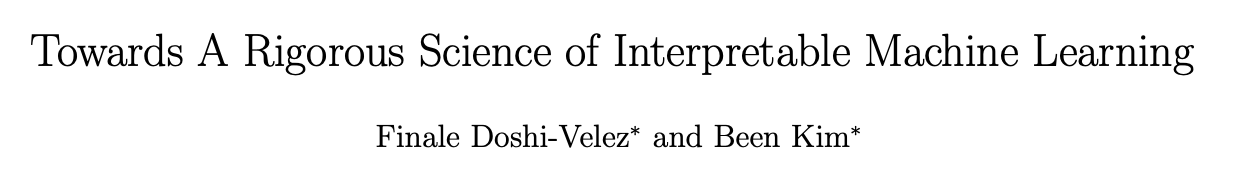
\includegraphics[width=0.9\paperwidth]{general_figures/doshi-velez_kim}

  \begin{itemize}
  \item Understanding: Debugging
  \item Trust: Does the user believe the system
  \item Simulation: Can the user recreate the system
  \item Safety / Ethics: Does the system protect/hurt people
  \item Mismatched Objectives: How do you balance with accuracy
    \only<2->{\item \alert<2>{Augmentation}}
  \end{itemize}

  \begin{center}
    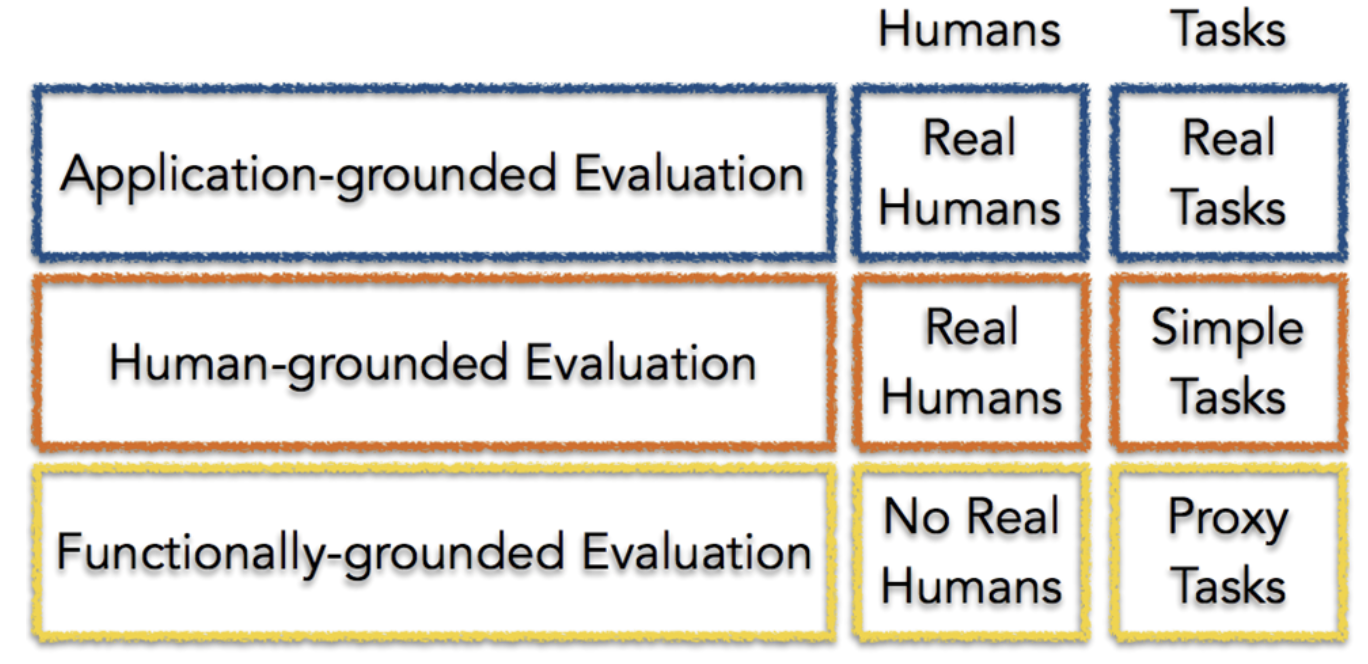
\includegraphics[width=0.5\paperwidth]{general_figures/interpretability_hierarchy}
    \end{center}
\end{frame}


\fsi{general_figures/chenhao_tutorial}{If you want to know more}

\begin{frame}
\frametitle{Unsupervised Methods: Dealing with the Deluge}

\begin{columns}

\column{.5\linewidth}

Every second \dots
\begin{itemize}
\item 3,400,00 e-mails sent
\item 740,741 WhatsApp messages sent
  \item 54,977 Facebook posts  
  \item 5,700 \sout{tweets} Xeets are \sout{tweeted} Xeeted
    \item 4,595 SMS Messages
    \end{itemize}
    (From Techcrunch, Zephoria, Intel)
\pause

\begin{block}{Unstructured}
  No XML, no semantic web, no annotation.  Often just raw text.
\end{block}

\column{.5\linewidth}

\only<3->{
Common task: what's going on in this dataset.
\begin{itemize}
   \item Intelligence analysts
   \item Brand monitoring
   \item Journalists
   \item Humanists
\end{itemize}
}
\only<4>{
\centering
Common solution: unsupervised machine learning (topic models)
}

\end{columns}

\end{frame}

\begin{frame}

\begin{center}
\frametitle{What does a Topic Model do?}
From an \textbf<1>{input corpus} and number of topics \textbf<1>{$K$} $\rightarrow$ \textbf<2>{words to topics} \\
\only<1>{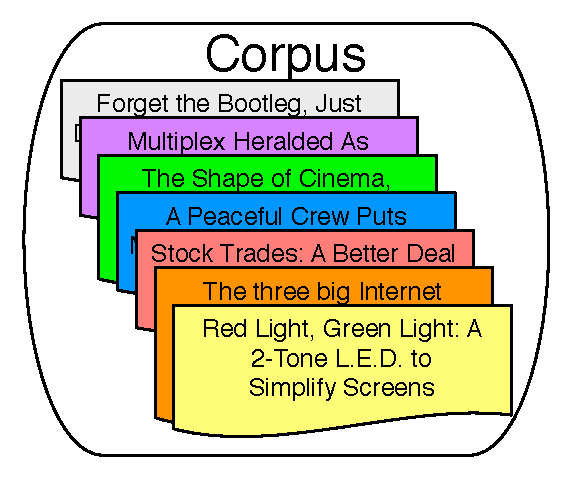
\includegraphics[width=0.6\linewidth]{reading_tea_leaves/figures/heldout_0} }
\only<2>{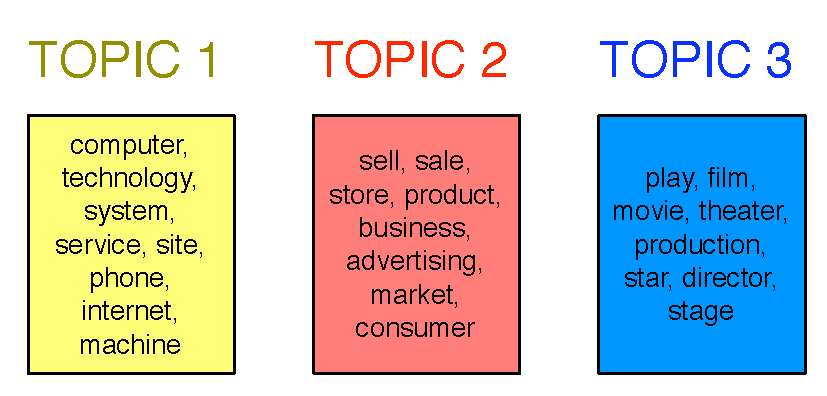
\includegraphics[width=0.9\linewidth]{reading_tea_leaves/figures/nyt_topics_wide}}
%\only<3>{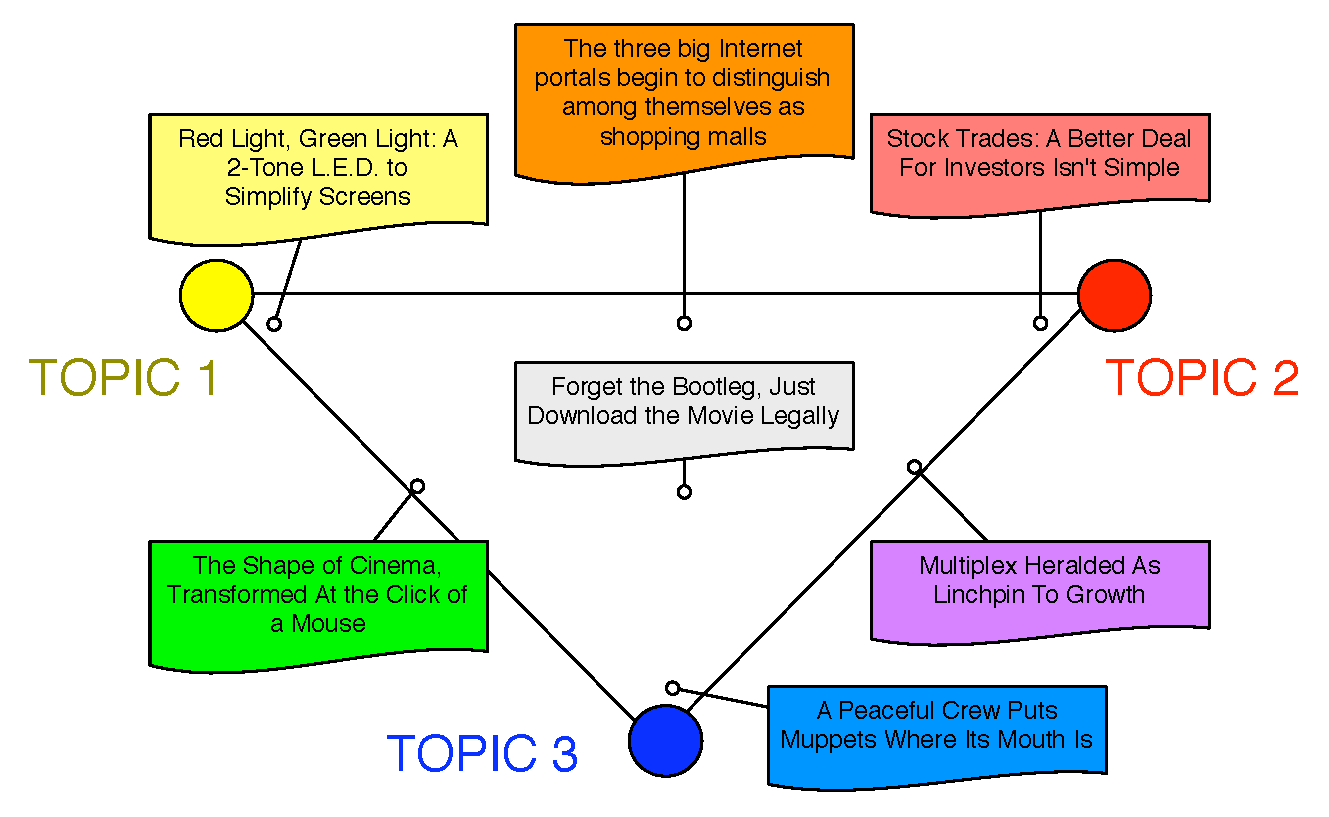
\includegraphics[width=0.9\linewidth]{topic_models/nyt_documents}}
\end{center}

\end{frame}


\begin{frame}{Evaluating Topic Models}

\begin{columns}

\column{.6\linewidth}
\begin{block}{ Reading Tea Leaves: How Humans Interpret Topic Models}
Jonathan Chang, Jordan Boyd-Graber, Chong Wang, Sean Gerrish, and David
M. Blei. Reading Tea Leaves: How Humans Interpret Topic Models. Neural
Information Processing Systems, 2009.
\end{block}

\column{.3\linewidth}
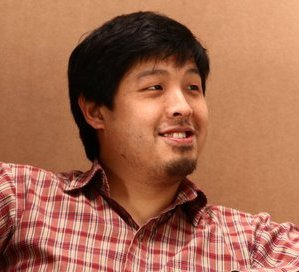
\includegraphics[width=.8\linewidth]{general_figures/jonathan}

\end{columns}

\end{frame}



\frame{
\frametitle{Evaluation}
\begin{center}
%\only<1>{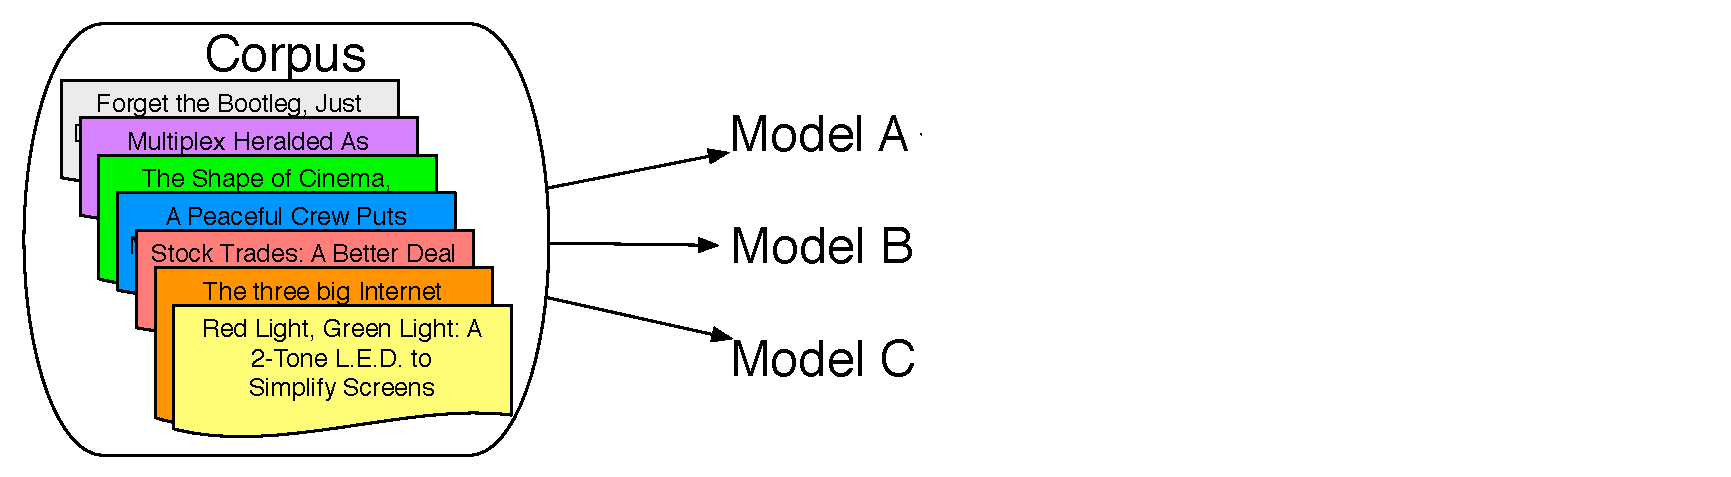
\includegraphics[width=0.9\linewidth]{reading_tea_leaves/figures/heldout_1} }
\only<1>{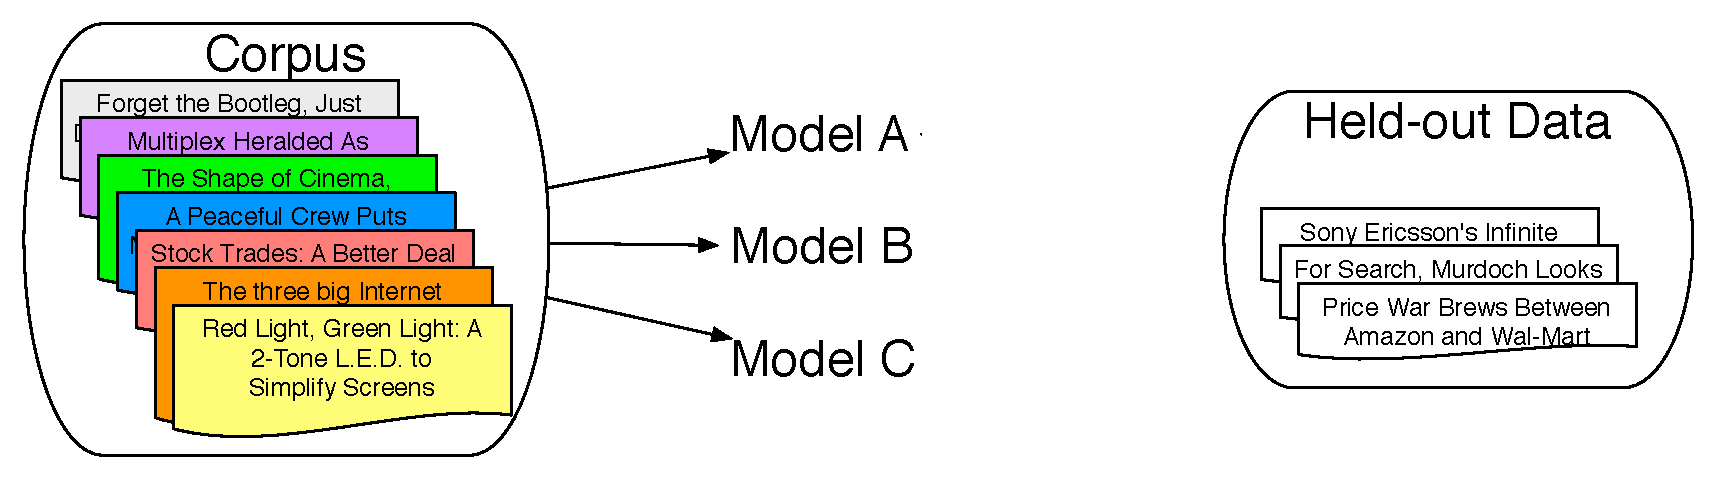
\includegraphics[width=\linewidth]{reading_tea_leaves/figures/heldout_2} }
%\only<3>{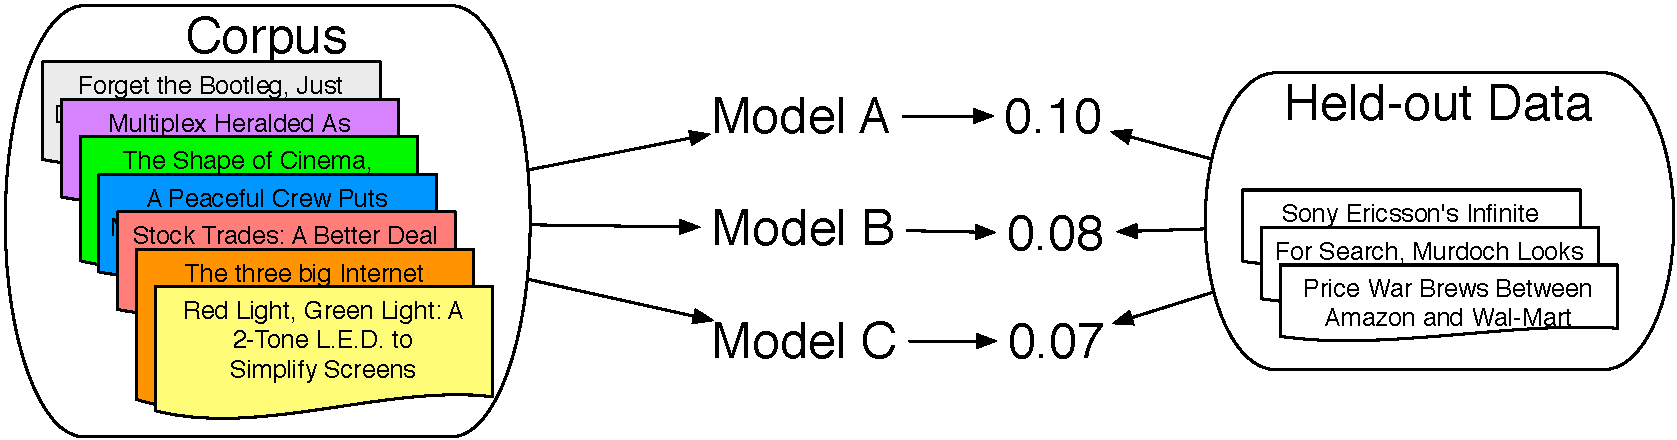
\includegraphics[width=\linewidth]{reading_tea_leaves/figures/heldout_3} }
\only<2>{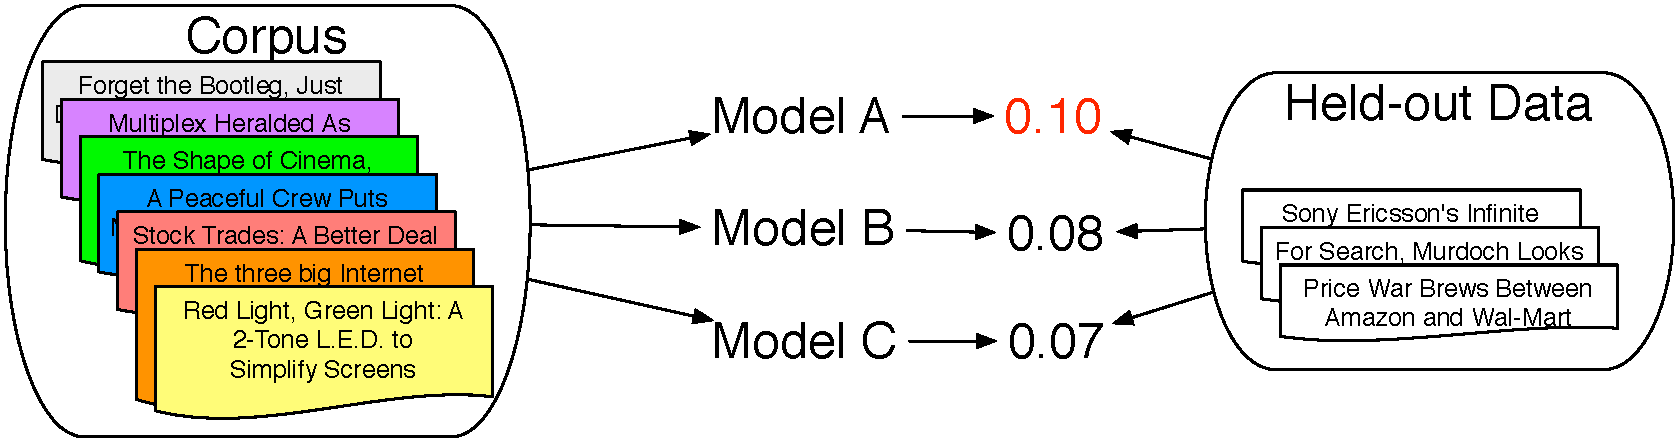
\includegraphics[width=\linewidth]{reading_tea_leaves/figures/heldout_4}  \\
	\large Measures predictive power (likelihood)}
\end{center}
}

\begin{frame}{Likelihood Computation}

  \begin{equation}
    P(\alert<5>{\mathcal{W}} \g \alert<2>{\mathcal{W}'}) = \int{ P( \alert<5>{\mathcal{W}} \g \alert<4>{\Phi},
      \alpha ) P(\phi \g \mathcal{W'}, \alert<3>{\alpha}) d\alert<4>{\Phi} } 
  \end{equation}

  \begin{itemize}
  \item \alert<2>{Training data}
    \item \alert<3>{Hyperparameters}
    \item \alert<4>{Latent variables (topics)}
      \item \alert<5>{Held out data}
  \end{itemize}
  
\end{frame}


\begin{frame}{But we don't use topic models for prediction!}

\gfxs{autocomplete}{.8}

\end{frame}

\frame{
\frametitle{Qualitative Evaluation of the Latent Space}

\begin{center}
\only<1>{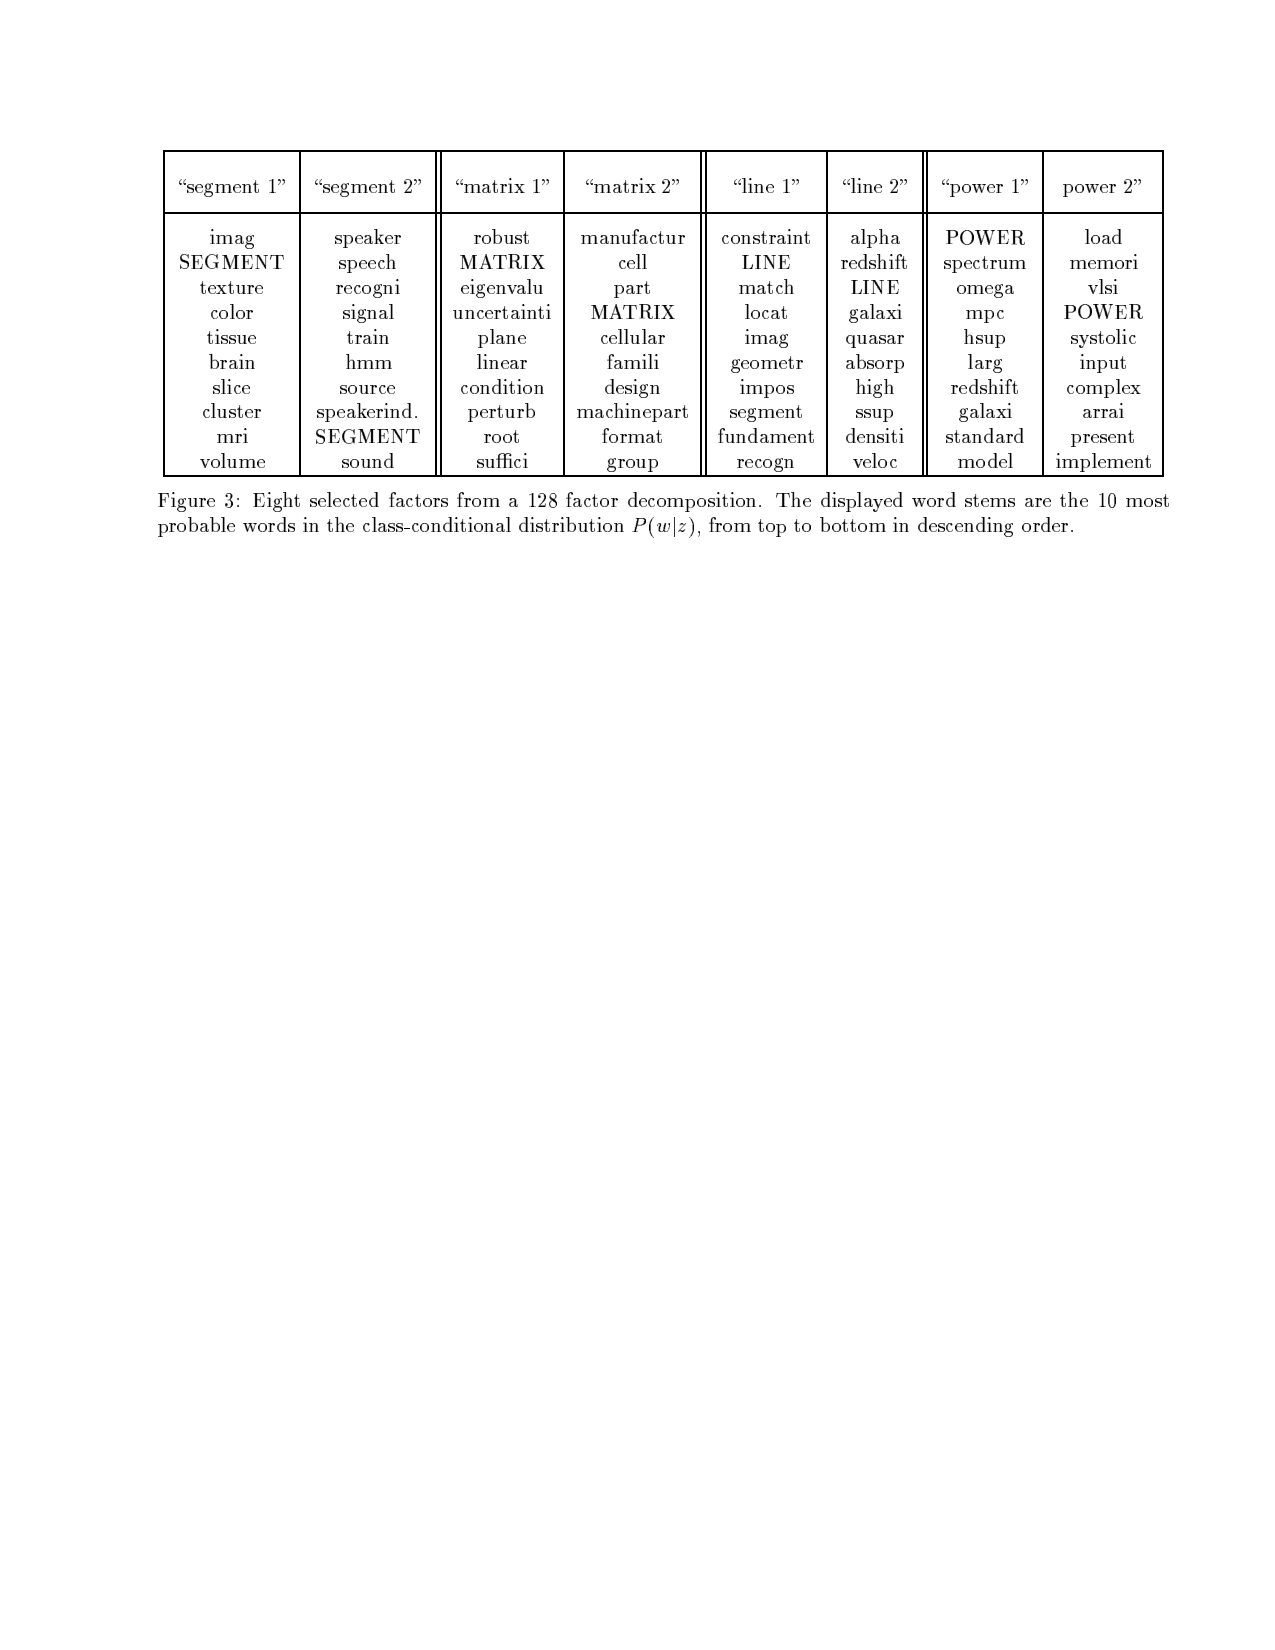
\includegraphics[width=0.9\linewidth]{reading_tea_leaves/topics_from_papers/1} \\ \cite{hofmann-99} }
\only<2>{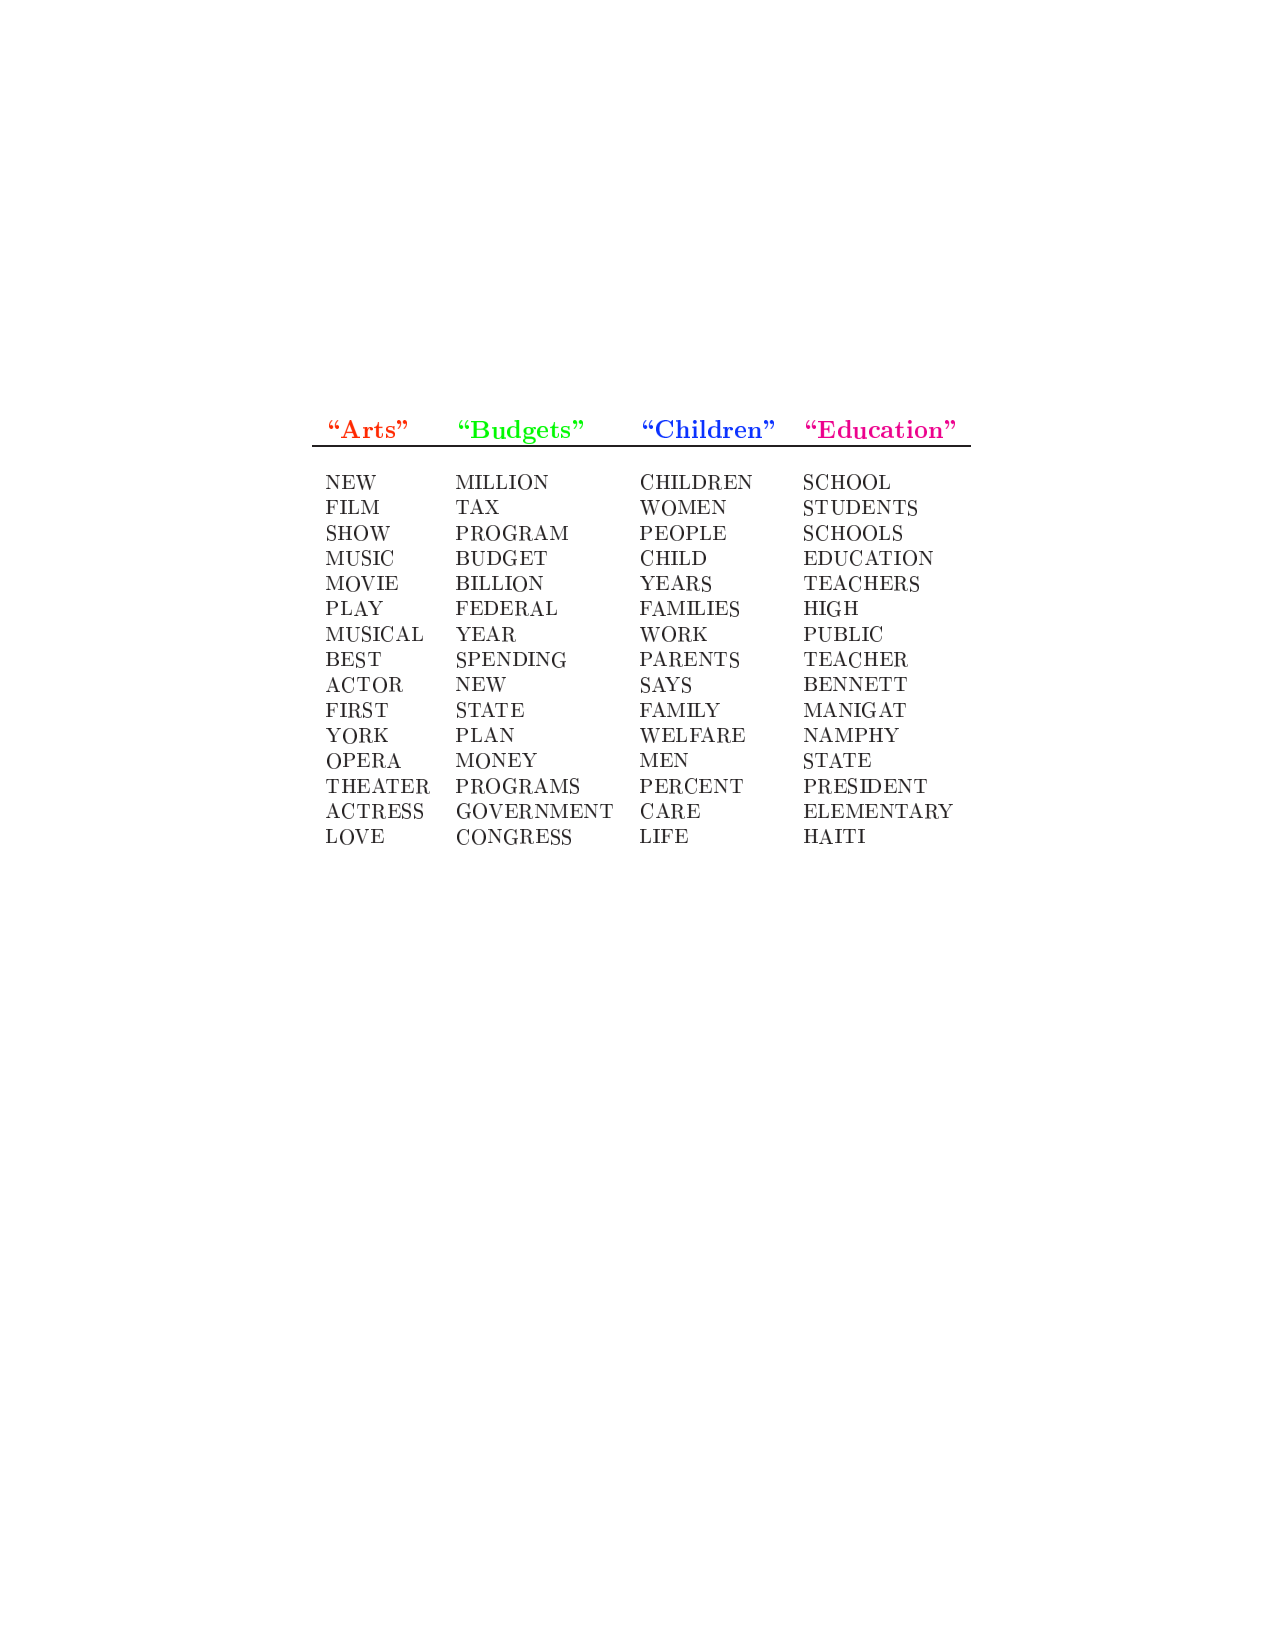
\includegraphics[width=0.7\linewidth]{reading_tea_leaves/topics_from_papers/2} \\ \cite{blei-03} }
\only<3>{
\includegraphics[width=0.7\linewidth]{reading_tea_leaves/topics_from_papers/3} \\ \cite{mimno-09} }
\only<4>{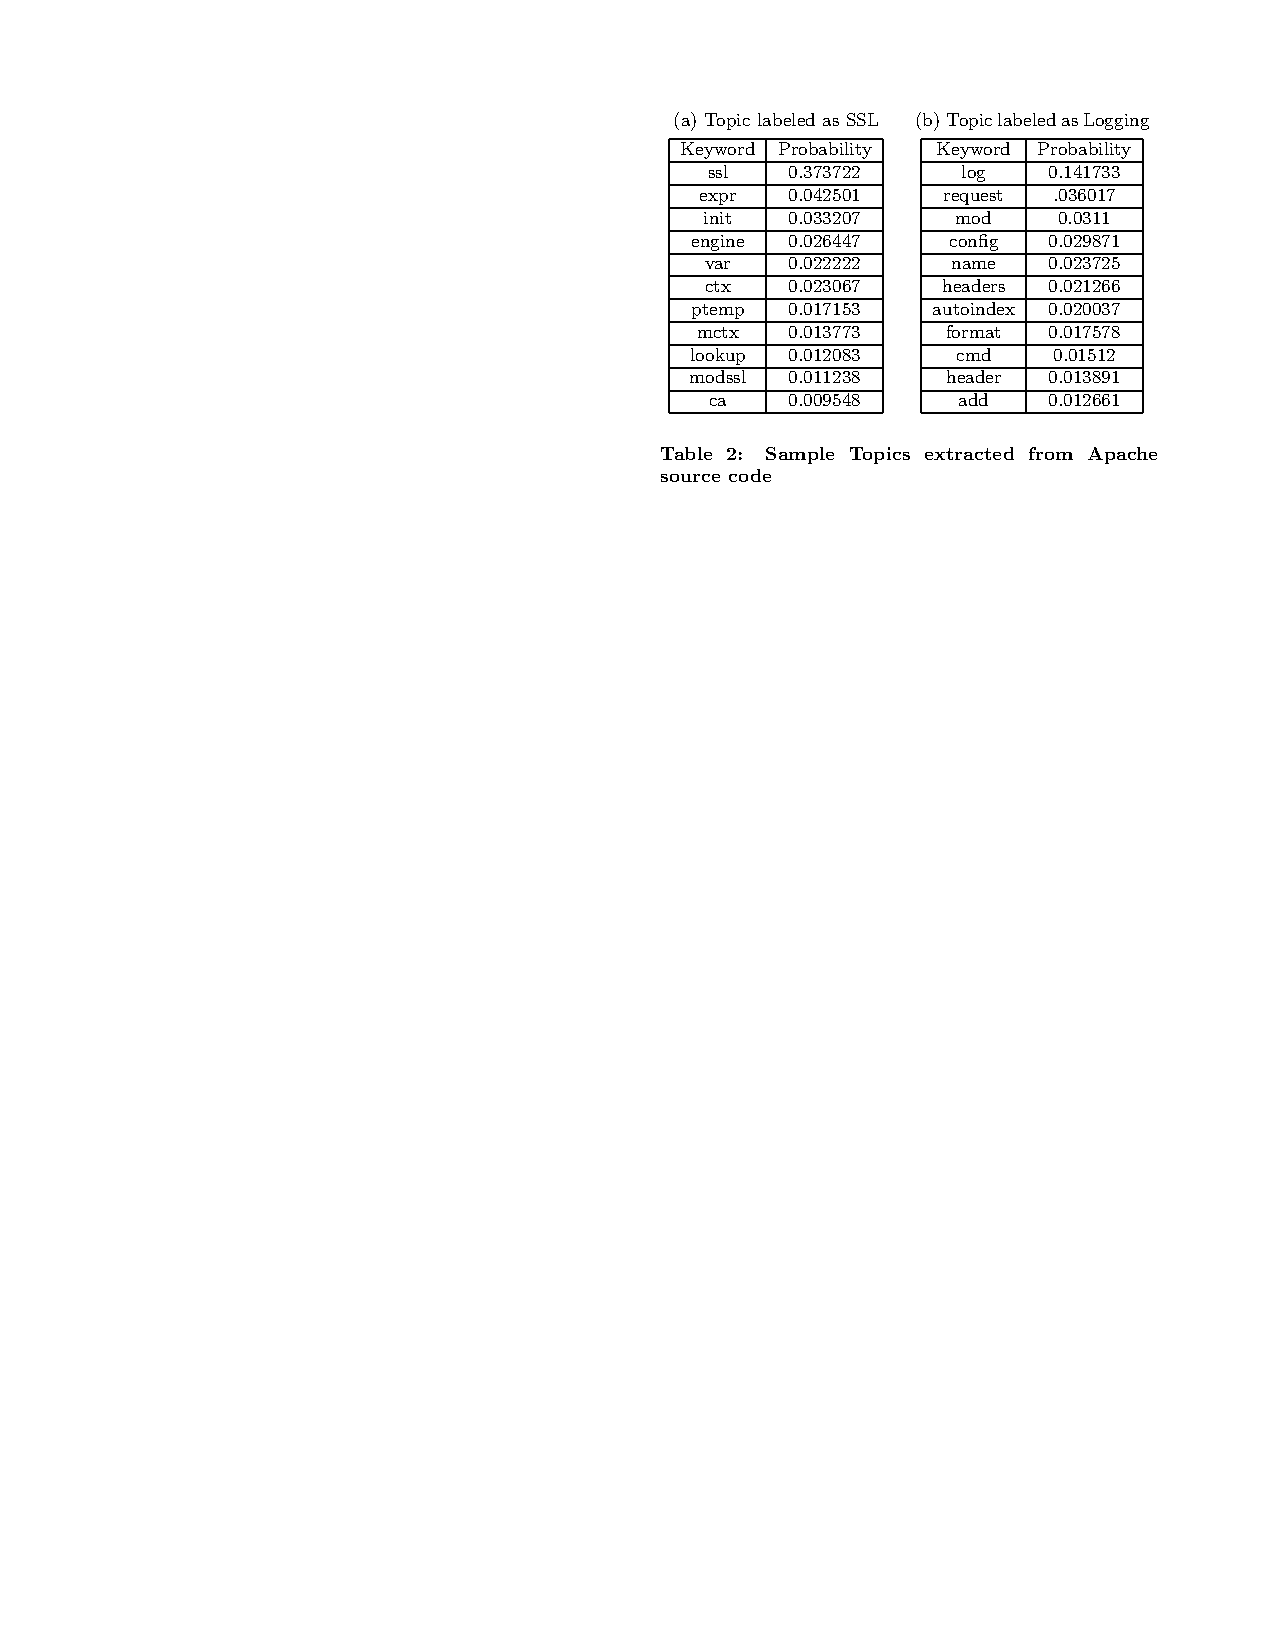
\includegraphics[width=0.7\linewidth]{reading_tea_leaves/topics_from_papers/4}
  \\ \cite{maskeri-08} }
\end{center}
}

\frame{
  \frametitle{Word Intrusion}

  \begin{itemize}
    \item Take the highest probability words from a topic

      \begin{block}{Original Topic}
        dog \\ cat \\ \only<2->{\alert<2->{apple} \\ } horse \\ pig \\ cow
      \end{block}

\only<2->{    \item \alert<2>{Intruder: high probability word from another topic}}
\pause
\item User's goal is to understand theme: can the user come to the
  same conclusion as the computer
  \end{itemize}
}

\frame{
\frametitle{Whom do we ask?}
\begin{columns}[c]


\column{0.45\linewidth}

\begin{block}{Then}
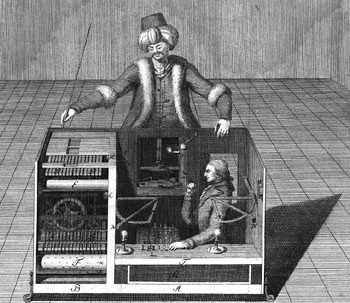
\includegraphics[width=0.95\linewidth]{evocation/figures/mechanical_turk_old}
\end{block}


\column{0.45\linewidth}

\begin{block}{Now}
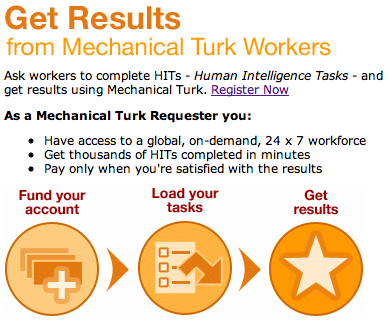
\includegraphics[width=0.95\linewidth]{evocation/figures/mechanical_turk_new}
\end{block}

\end{columns}
}


\frame{
\frametitle{Interpretability and Likelihood}


\begin{center}
\only<1>{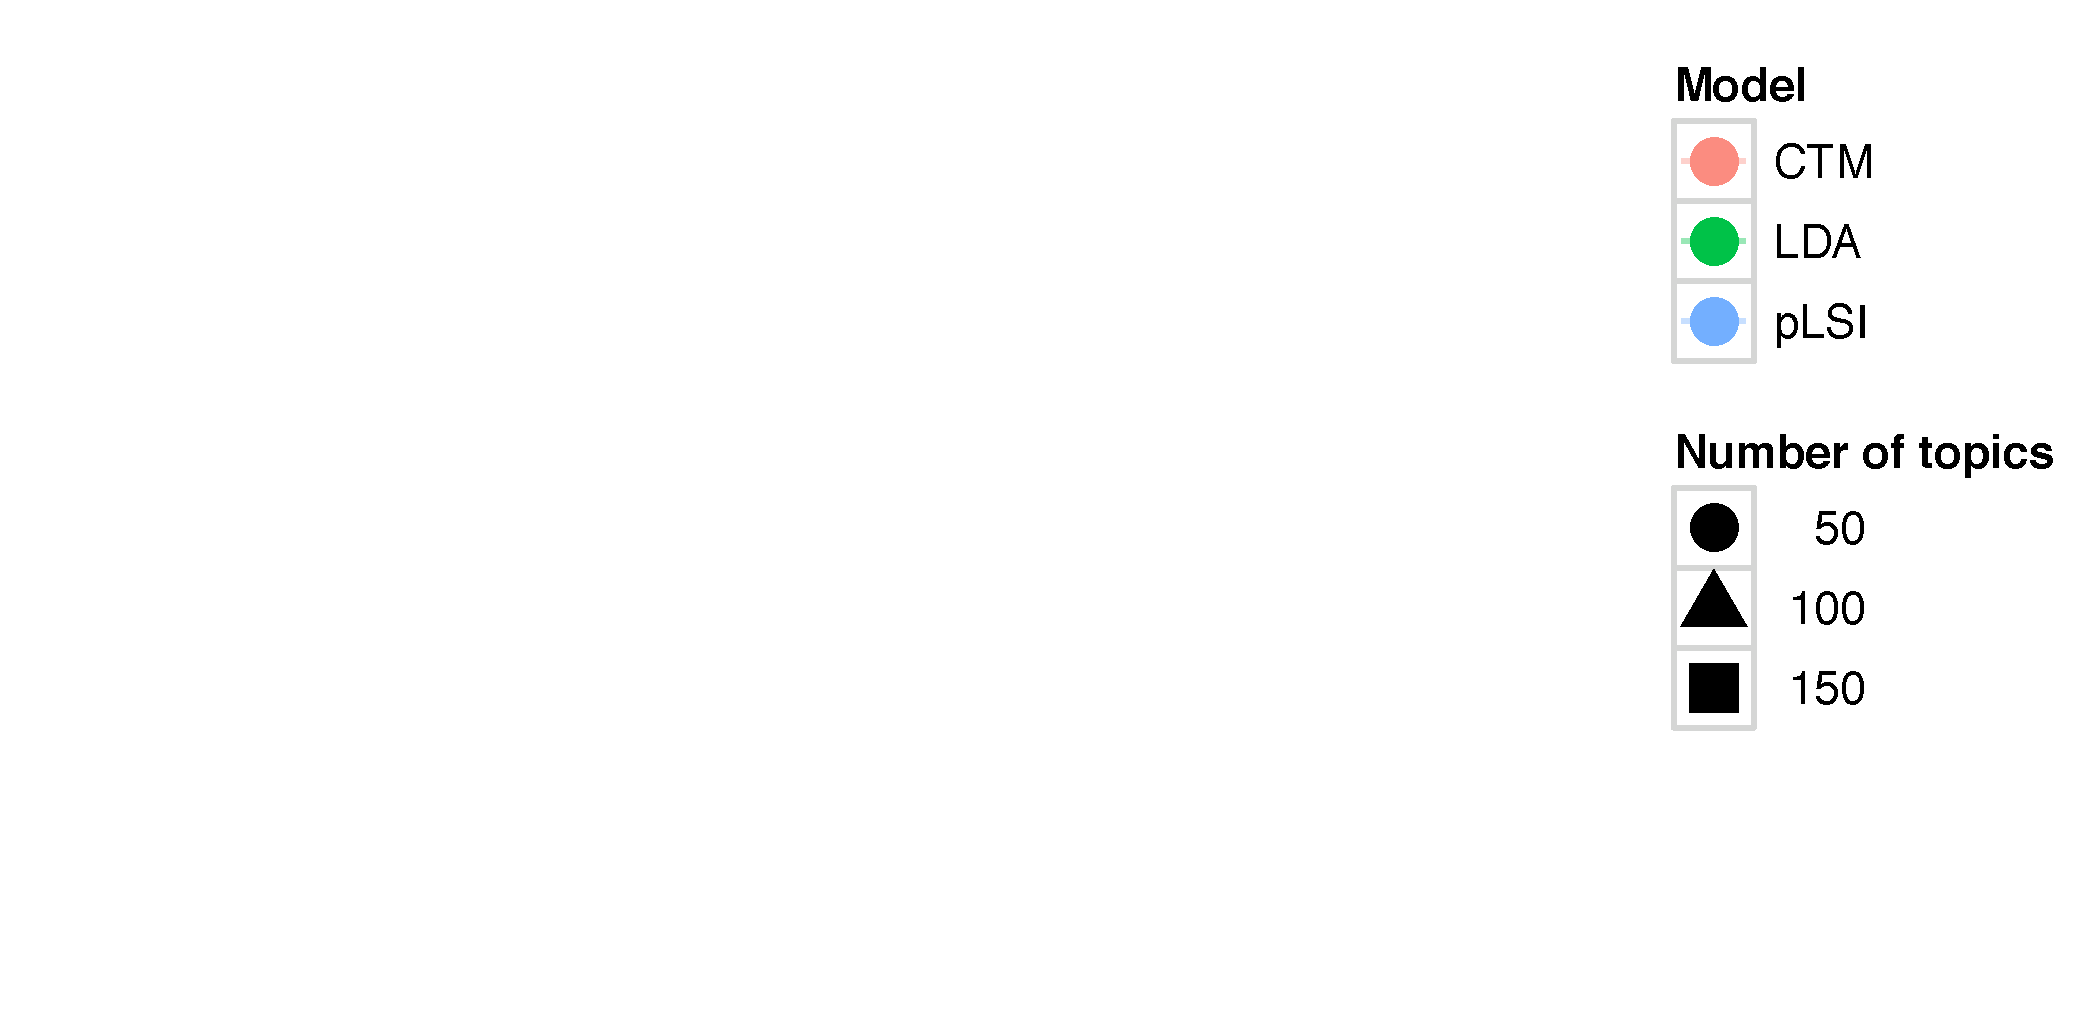
\includegraphics[width=.8\paperwidth]{reading_tea_leaves/figures/prec_ll_1}}
\only<2>{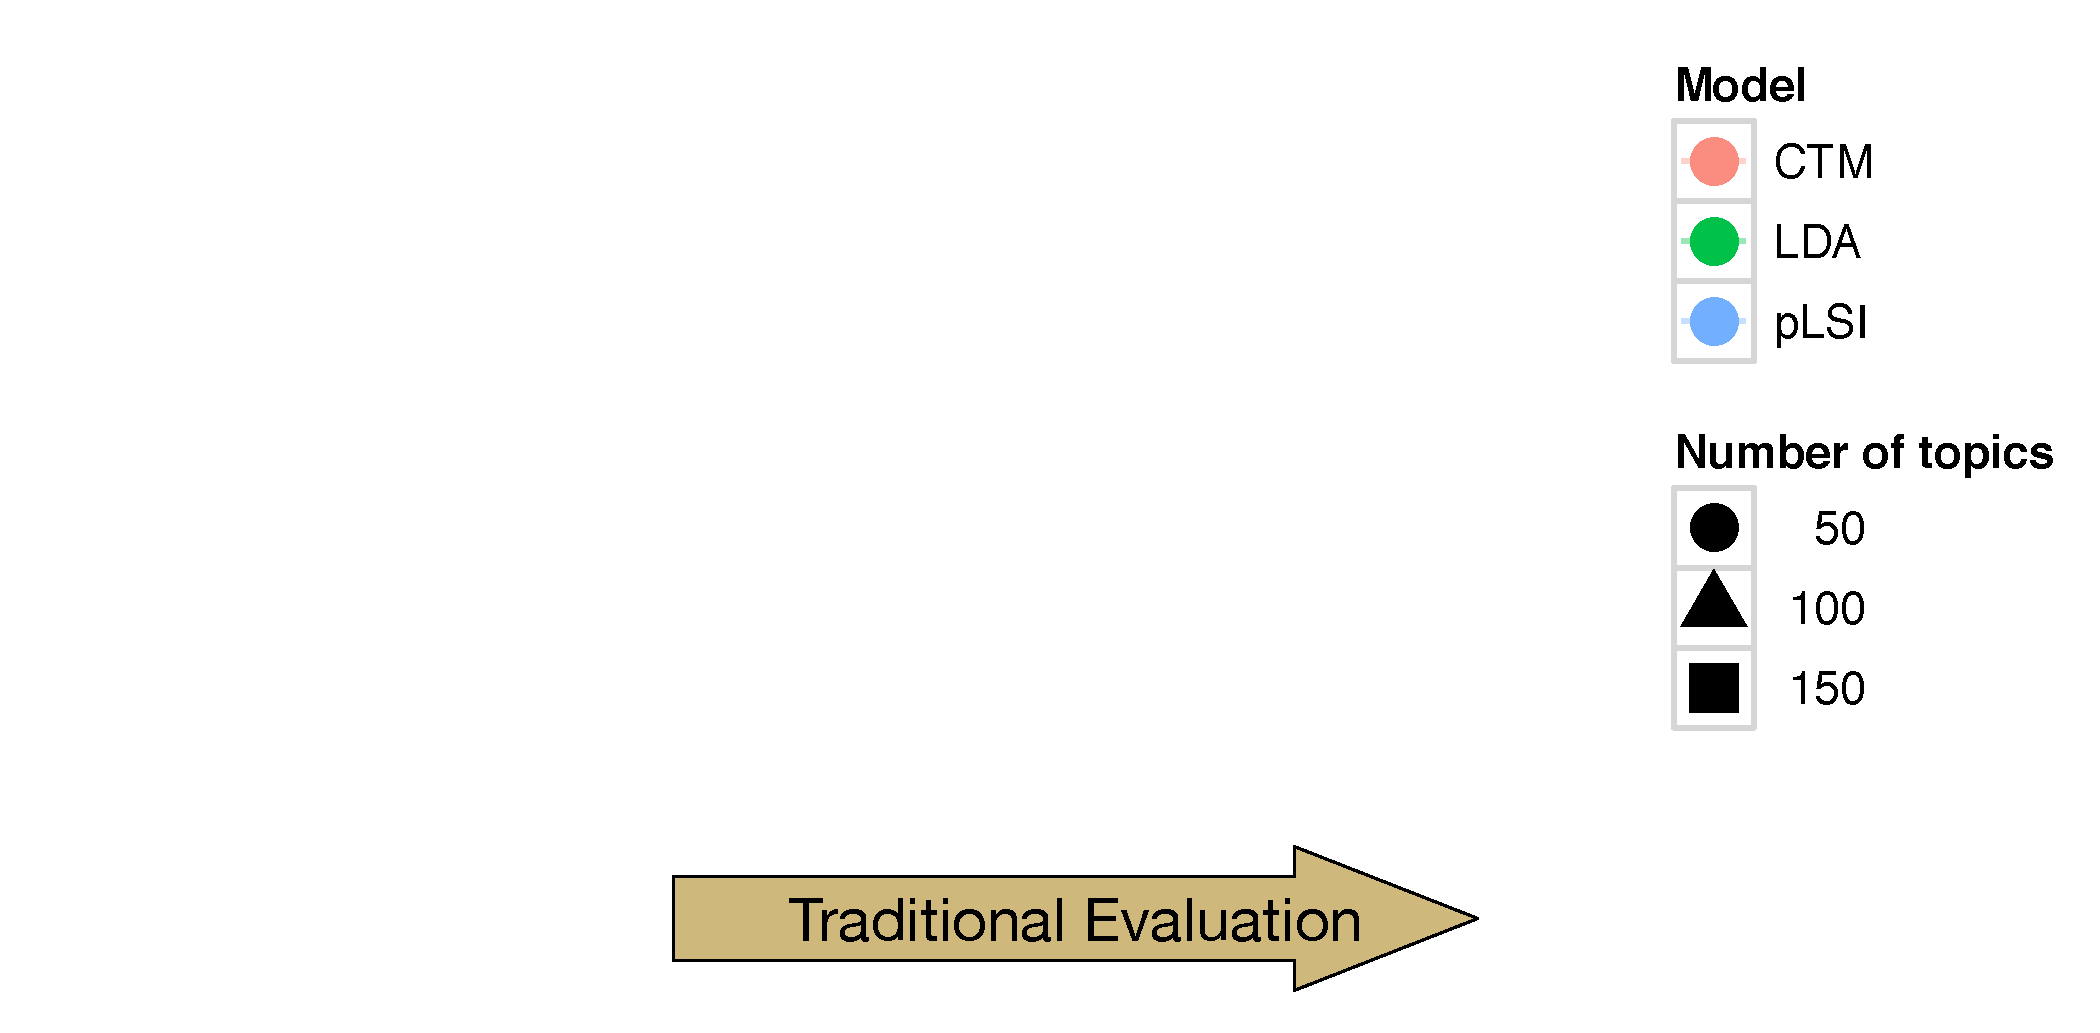
\includegraphics[width=.8\paperwidth]{reading_tea_leaves/figures/prec_ll_2}}
\only<3>{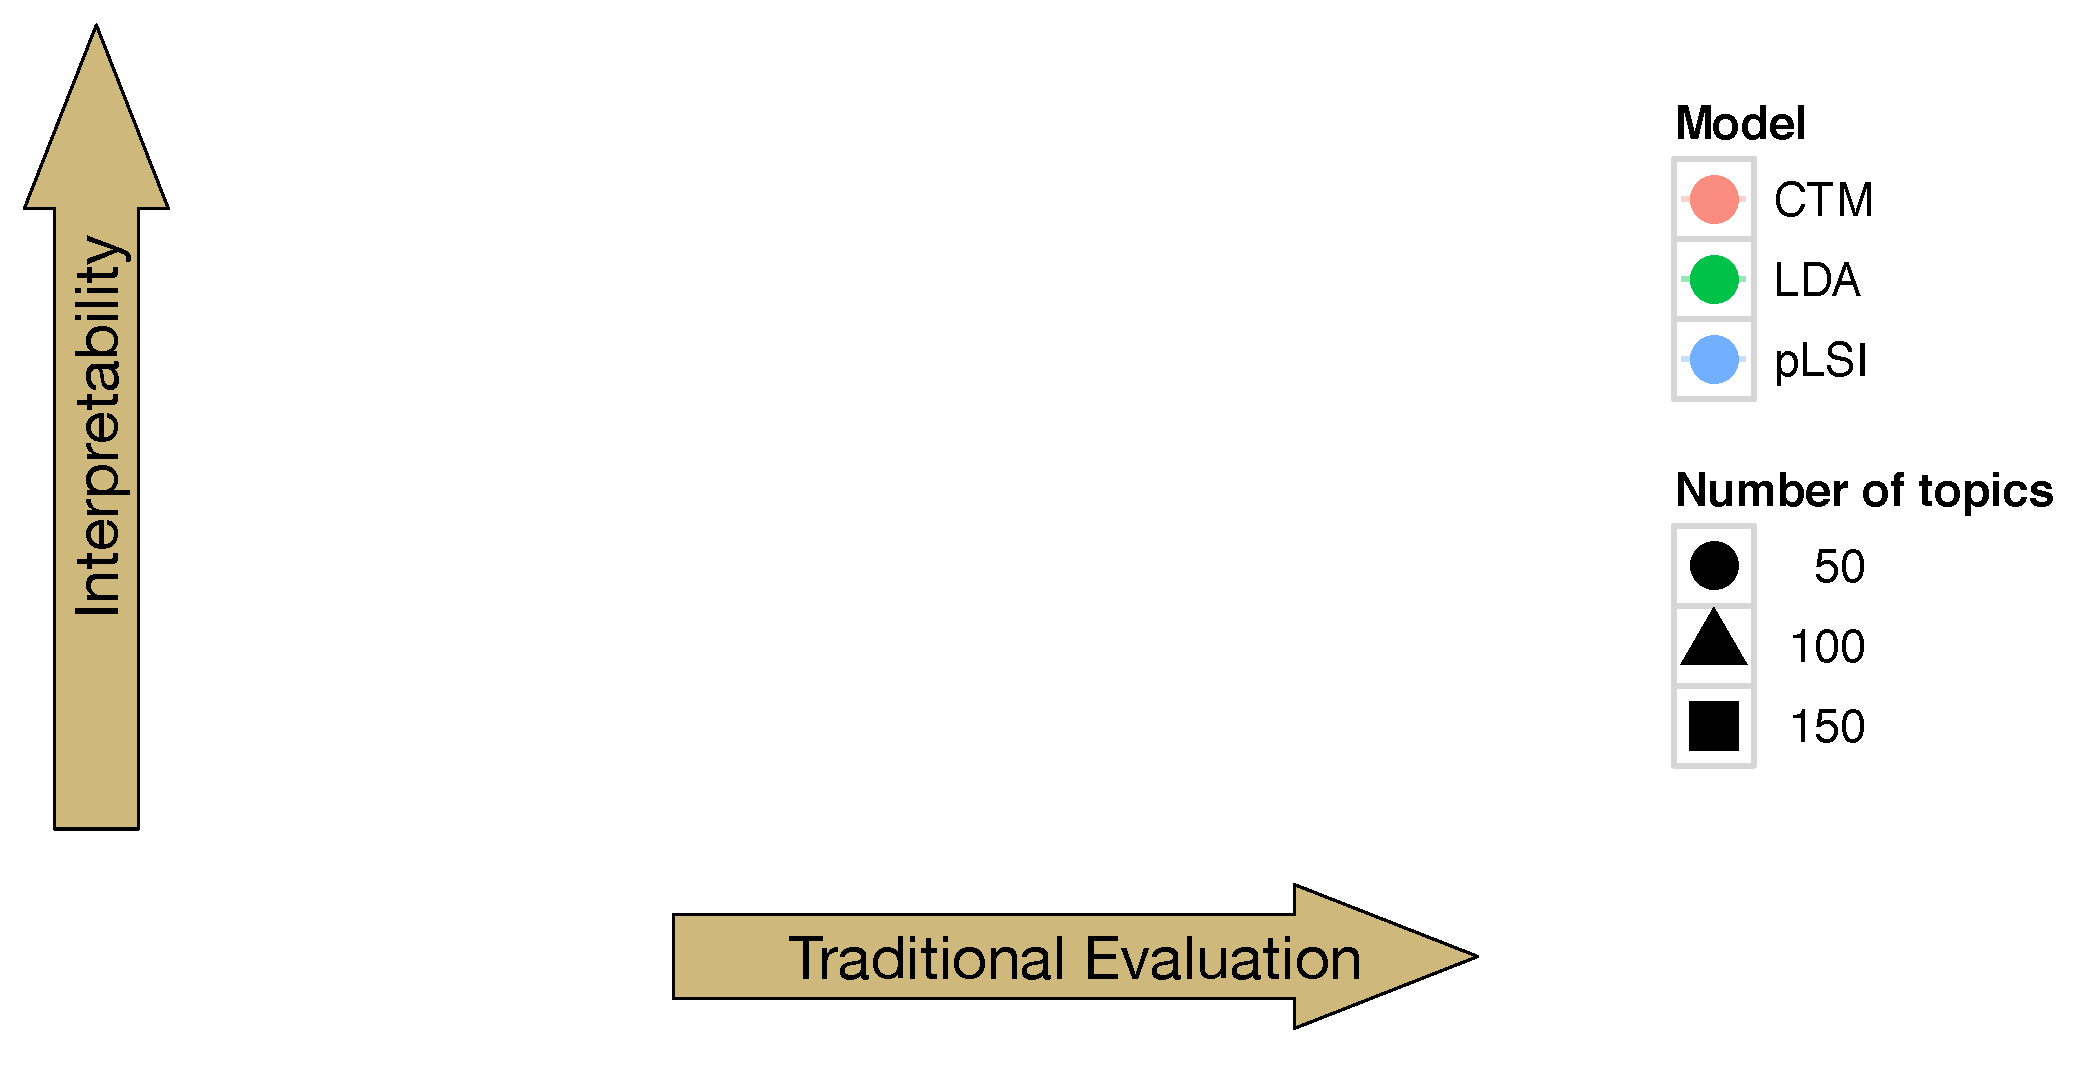
\includegraphics[width=.8\paperwidth]{reading_tea_leaves/figures/prec_ll_3}}
\only<4>{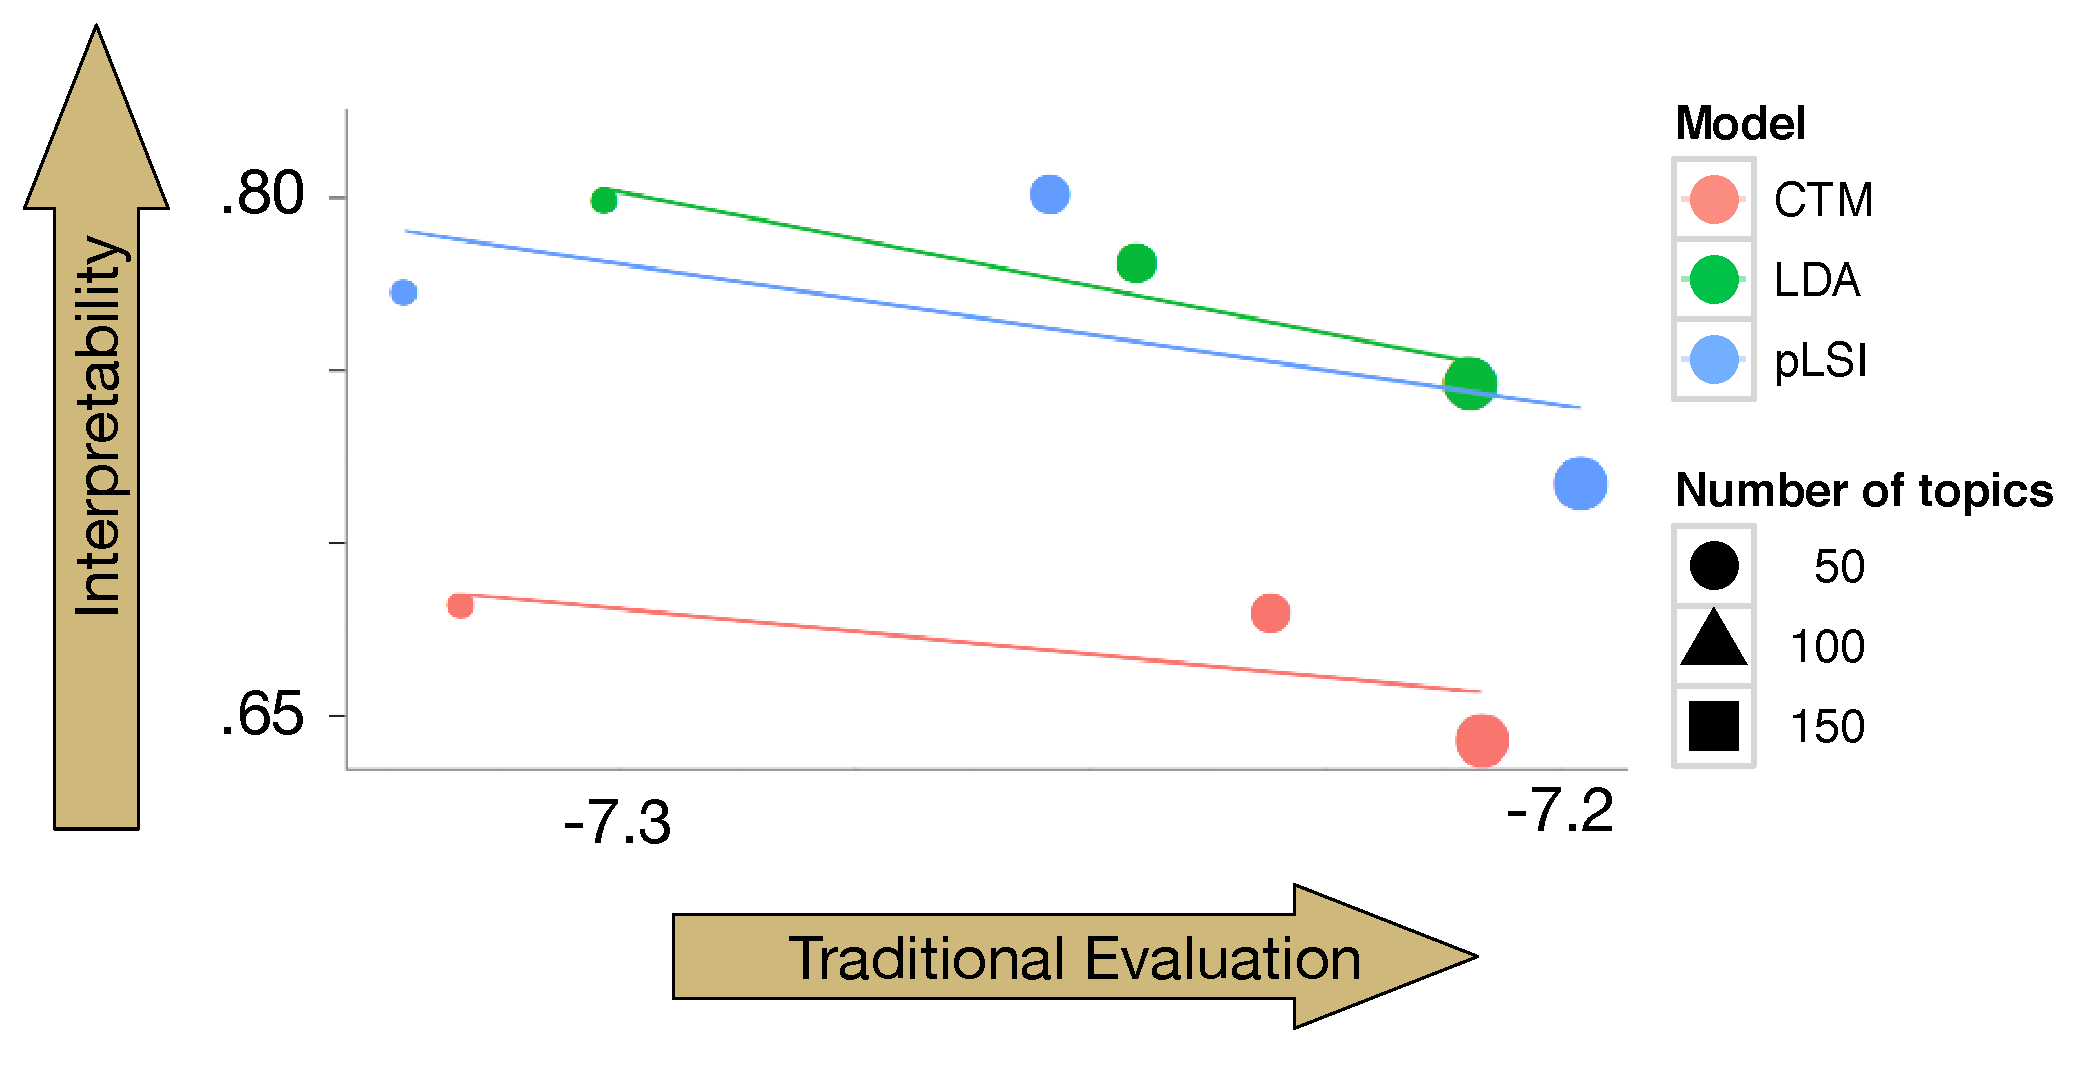
\includegraphics[width=.8\paperwidth]{reading_tea_leaves/figures/prec_ll_4}}
\only<4>{\\ Within a model, higher likelihood $\not =$ higher interpretability}
\end{center}
}

\begin{frame}{Machine Reading Tea Leaves}
  
\includegraphics[width=.8\paperwidth]{reading_tea_leaves/machine_reading_tea_leaves}

  \begin{itemize}
  \item Take a reference corpus, compute probability of words in that corpus
  \item For a topic, take all pairs of words $w_i$, $w_j$ in the top
    $n$ words
  \item OC-Auto-NPMI
    \begin{equation}
      \sum_{j=2}^{N}\sum_{i=1}^{j-1}{{ \frac{\log \frac{P(w_j,
          w_i)}{P(w_i)P(w_j)}}{-\log P(w_i, w_j)}}}
    \end{equation}
    \item Words that appear near each other in documents more than
      their natural frequency
  \end{itemize}
  
\end{frame}


\begin{frame}{Since then \dots}

  \begin{itemize}
    \item Used to manage \abr{nih}'s funding portfolio~\cite{talley-11}
    \item \alert<2>{Others have discovered automatic methods that uncover the same properties}~\cite{newman-10,mimno-11}
    \item Evaluations for structured topics and
      phrases~\cite{lindsey-12,weninger-12}
      \item We developed ways to fix topic models with tree-structured
        priors~\cite{hu-14} and spectral algorithms~\cite{Lund-17}
      \item Extending to multiple users~\cite{Felt-15}
        \pause
        \item Neural networks everywhere
  \end{itemize}

\end{frame}

\fsi{general_figures/w2v_flow}{word2vec (Mikolov et al., 2013)}

\begin{frame}{You know what's cool?}

  \begin{columns}
    \column{.4\linewidth}
    \gfxt{drake_neural}{.9}
    \column{.6\linewidth}
  \begin{itemize}
  \item Autoencoding Variational Inference for Topic Models~\cite{srivastava-17}
    \item Embedded Topic Model: combine word representations into
      document representations~\cite{dieng-20}
    \item Contextualized Topic Model: Reproduce word--document
      coocurrence with \abr{bert}~\cite{bianchi-21}
    \pause
  \item Trivia: word2vec with dimension~$k$ is factorizing~\cite{levy-14}
    \begin{equation}
      \mbox{PMI}(w_i, c_j) - \log k
    \end{equation}
  \end{itemize}

  \end{columns}
\end{frame}

\begin{frame}{}

  \begin{columns}
    \column{.4\linewidth}
    \begin{center}
        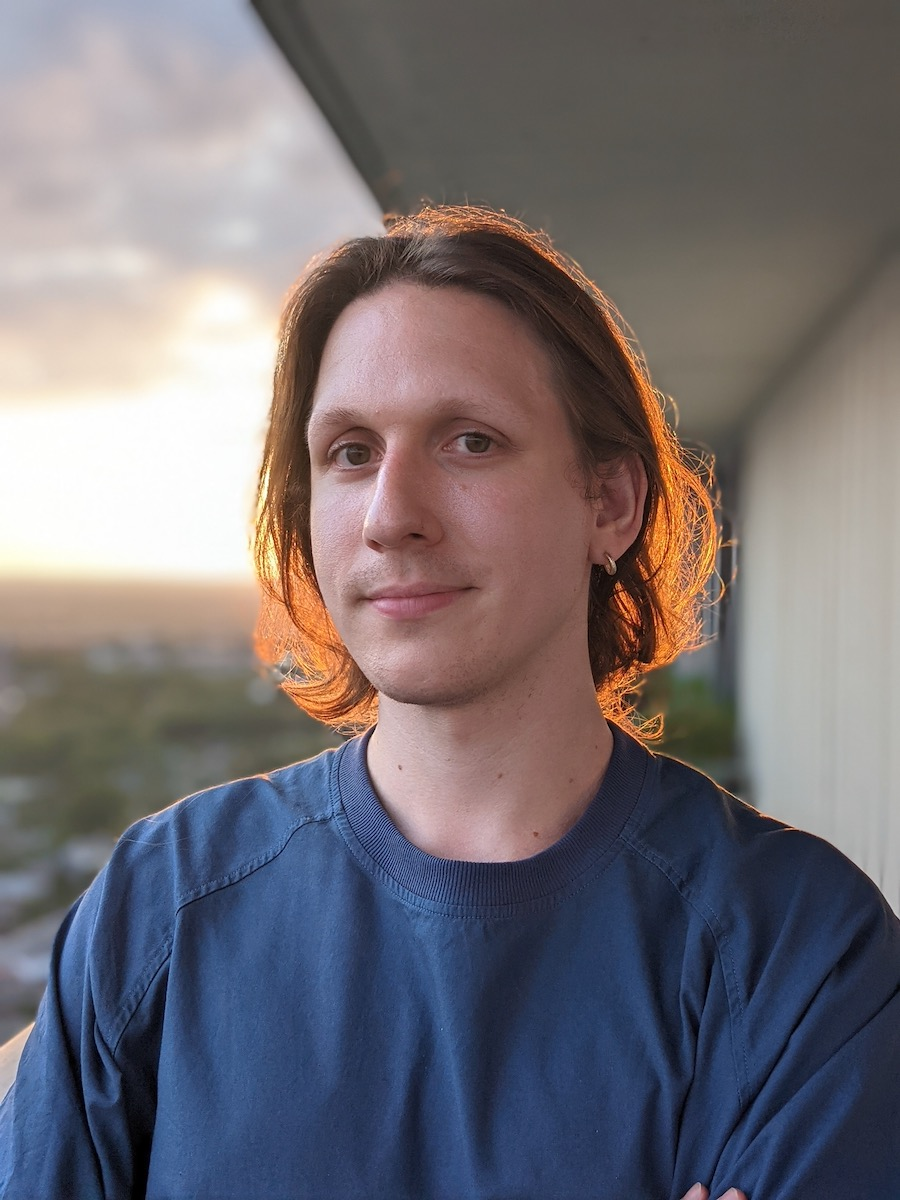
\includegraphics[width=0.8\linewidth]{general_figures/alexander}
        \end{center}
    \column{.6\linewidth}
    \begin{block}{\href{http://umiacs.umd.edu/~jbg//docs/2021_neurips_incoherence.pdf}{Is Automated Topic Evaluation Broken? The Incoherence of Coherence}}
      \href{https://alexanderhoyle.com/}{Alexander Miserlis Hoyle},
      Pranav Goel, Andrew Hian-Cheong, Denis Peskov, Jordan
      Boyd-Graber, and Philip Resnik.
      \emph{Neural Information Processing Systems}, 2021
        \end{block}

  \end{columns}
\end{frame}

\begin{frame}{Is Automatic Coherence Good Enough?}

  \begin{table}
	\centering
		\resizebox{\textheight}{!}{
			\begin{tabular}{lllllllllll}
				\toprule
				Source & Human        & Perplexity & Coherence       & Implementation & Ref. Corpus   & Consistent & Hparam   & >1 run /     & LDA             & Baseline \\
				& Evals?       &            &                 & Specified      & Specified ?   & Preproc?    & search? & err. bars?   & Implementation? & w/in 2 yr?\\
				\midrule
~\cite{Bianchi2020PretrainingIA} & \alert<2>{No} & No & \abr{npmi}, Embed-sim & None & Internal, External-GoogleNews & Yes & No & Yes & Variational & No\\
~\cite{zhao2021neural} & \alert<2>{No} & No & \abr{npmi} & Palmetto & No & Unclear & No & Yes & N/A & Yes\\
~\cite{Feng2020ContextRN} & \alert<2>{No} & Yes & \abr{npmi} & None & No & Yes & No & No & N/A & Yes\\
~\cite{hoyle-etal-2020-improving} & \alert<2>{No} & No & \abr{npmi} & In paper & External \abr{nyt}, Internal & No & Yes & Yes & N/A & Yes\\
~\cite{Hu2020NeuralTM} & \alert<2>{No} & No & $C_p$, $C_a$, \abr{npmi} & Palmetto & External \abr{wiki} & No & Likely no & No & Sampling & Yes\\
~\cite{Isonuma2020TreeStructuredNT} & \alert<2>{No} & Yes & \abr{npmi} & None & No, likely external & Unclear & No & No & Sampling & No\\
~\cite{Joo2020DirichletVA} & \alert<2>{No} & Yes & \abr{npmi} & None & No, likely internal & No & Likely yes & Yes & N/A & Yes\\
~\cite{Lin2020CopulaGN} & \alert<2>{No} & Yes & \abr{npmi} & None & No, likely internal & Unclear & Yes & Yes & N/A & Yes\\
~\cite{Ning2020NonparametricTM} & \alert<2>{No} & Yes & \abr{npmi} & Lau github & No & Yes & Likely no & Yes & Variational & No\\
~\cite{Panwar2020TANNTMTA} & \alert<2>{No} & No & \abr{npmi} & Lau github & No & Yes & Likely no & No & Sampling & Yes\\
~\cite{Rezaee2020ADV} & \alert<2>{No} & No & N/A & N/A & N/A & Yes & Likely no & Yes & Variational & No\\
~\cite{Thompson2020TopicMW} & \alert<2>{No} & No & Coherence, \abr{pmi} & In paper & External \abr{nyt} & No & No & Yes & Sampling & No\\
~\cite{Tian2020LearningVM} & \alert<2>{No} & Yes & \abr{npmi} & None & No & No & Yes & No & Variational & Yes\\
~\cite{Wang2020NeuralTM} & \alert<2>{No} & No & $C_p$, $C_a$, \abr{npmi}, UCI & Palmetto & No & No & No & No & Sampling & Yes\\
~\cite{Wu2020NeuralMC} & \alert<2>{No} & Yes & \abr{npmi} & None & No & No & Yes & No & N/A & Yes\\
~\cite{Wu2020ShortTT} & \alert<2>{No} & No & $C_v$ & Palmetto & No & Yes & No & No & Unspecified & Yes\\
~\cite{Yang2020GraphAT} & \alert<2>{No} & Yes & Coherence & In paper & No, likely internal & Yes & No & No & Unspecified & No\\
~\cite{Zhou2020NeuralTM} & \alert<2>{No} & No & \abr{npmi}, $C_p$ & Palmetto & External \abr{wiki} & No & Likely no & No & Unspecified & Yes\\
~\cite{burkhardtDecouplingSparsitySmoothness2019} & \alert<2>{No} & Yes & \abr{npmi} & None & No, likely internal & Unclear & Yes & No & Variational & Yes\\
~\cite{diengTopicModelingEmbedding2019} & \alert<2>{No} & Yes & Coherence & In paper & No, likely internal & Yes & No & No & Unspecified & No\\
~\cite{Gui2019NeuralTM} & \alert<2>{No} & No & $C_v$ & None & External \abr{wiki} & Yes & Likely no & No & Unspecified & Yes\\
~\cite{Gupta2019DocumentIN} & \alert<2>{No} & Yes & $C_v$ & Gensim & No, likely internal & Unclear & Likely no & No & N/A & No\\
~\cite{Gupta2019textTOvecDC} & \alert<2>{No} & Yes & $C_v$ & Gensim & No, likely internal & Unclear & Likely no & No & Sampling & Yes\\
~\cite{Lin2019SparsemaxAR} & \alert<2>{No} & Yes & PMI & In paper & No, likely external & Unclear & No & No & Variational & Yes\\
~\cite{Liu2019NeuralVC} & \alert<2>{No} & Yes & \abr{npmi} & Lau github & No, likely internal & Yes & No & No & Variational & Yes\\
~\cite{Nan2019TopicMW} & \alert<2>{No} & No & \abr{npmi} & None & No & No & No & No & Sampling & Yes\\
~\cite{Wang2019ATMAT} & \alert<2>{No} & No & $C_p$, $C_a$, UCI, \abr{npmi}, UMASS & Palmetto & No & No & No & No & Unspecified & Yes\\
~\cite{Card2018NeuralMF} & \alert<2>{No} & Yes & \abr{npmi} & In paper & External-gigaword & Yes & Likely yes & No & Sampling & Yes\\
~\cite{Ding2018CoherenceAwareNT} & \alert<2>{No} & Yes & \abr{npmi} & Lau github & No, likely external & No & Likely no & No & Sampling & Yes\\
~\cite{He2018InteractionAwareTM} & \alert<2>{No} & No & Coherence & None & No, likely internal & Yes & No & No & N/A & Yes\\
~\cite{Peng2018NeuralST} & \alert<2>{No} & Yes & N/A & N/A & N/A & Yes & Likely no & No & Variational & Yes\\
~\cite{Silveira2018TopicMU} & \alert<2>{No} & Yes & \abr{npmi} & Lau github & Internal & Yes & No & Yes & N/A & Yes\\
~\cite{Zhang2018WHAIWH} & \alert<2>{No} & Yes & N/A & N/A & N/A & Unclear & Likely no & No & N/A & Yes\\
~\cite{Zhao2018DirichletBN} & \alert<2>{No} & Yes & \abr{npmi} & Palmetto & External \abr{wiki} & Unclear & No & Yes & N/A & Yes\\
~\cite{Zhu2018GraphBTMGE} & \alert<2>{No} & No & Coherence & None & No, likely internal & Yes & Likely no & No & Variational & Yes\\
~\cite{Jung2017ContinuousST} & \alert<2>{No} & Yes & \abr{npmi}, \abr{PMI}, UMASS & None & No & Yes & No & No & Sampling & Yes\\
~\cite{Miao2017DiscoveringDL} & \alert<2>{No} & Yes & \abr{npmi} & In paper & No & No & Likely no & No & Variational & Yes\\
~\cite{Srivastava2017AutoencodingVI} & \alert<2>{No} & Yes & \abr{npmi} & None & No & Yes & No & No & Sampling & Yes\\
~\cite{Miao2016NeuralVI} & \alert<2>{No} & Yes & N/A & N/A & N/A & Yes & Likely no & No & Unspecified & Yes\\
~\cite{Nguyen2015ImprovingTM} & \alert<2>{No} & No & \abr{npmi} & Lau github & External \abr{wiki} & Yes & No & Yes & Sampling & No\\
				\bottomrule
			\end{tabular}
		}
	\caption{Papers used in meta-analysis}
\end{table}

\end{frame}

\fsi{reading_tea_leaves/incoherence/model_comparison_boxplot_0}{All that
passes automatic evaluations is not Gold}

\fsi{reading_tea_leaves/incoherence/model_comparison_boxplot_1}{All that
passes automatic evaluations is not Gold}

\fsi{reading_tea_leaves/incoherence/model_comparison_boxplot}{All that
passes automatic evaluations is not Gold}


\begin{frame}{What about Supervised Models?}

  \only<1>{
    \begin{columns}
      \column{.5\linewidth}
      \begin{block}{Unsupervised Methods}
        $p(z, x)$
      \end{block}
      \column{.5\linewidth}
      \begin{block}{Supervised Methods}
        $p(y \;|\; x)$
      \end{block}      
    \end{columns}

    \begin{itemize}
    \item Unsupervised methods \emph{discover} structure
    \item Supervised methods \emph{reproduce} correct answers
    \end{itemize}
  }

  
\only<2>{
\begin{center}
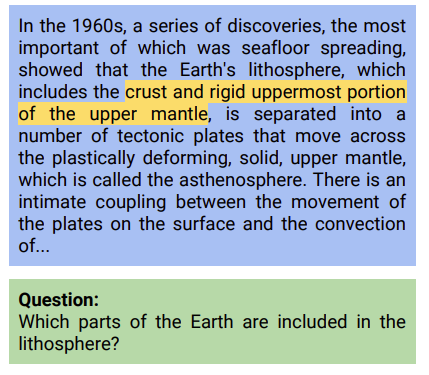
\includegraphics[width=.6\paperwidth]{qb/squad_ex}
\end{center}
}
\end{frame}


\begin{frame}[plain]
  \vspace{-2cm}
		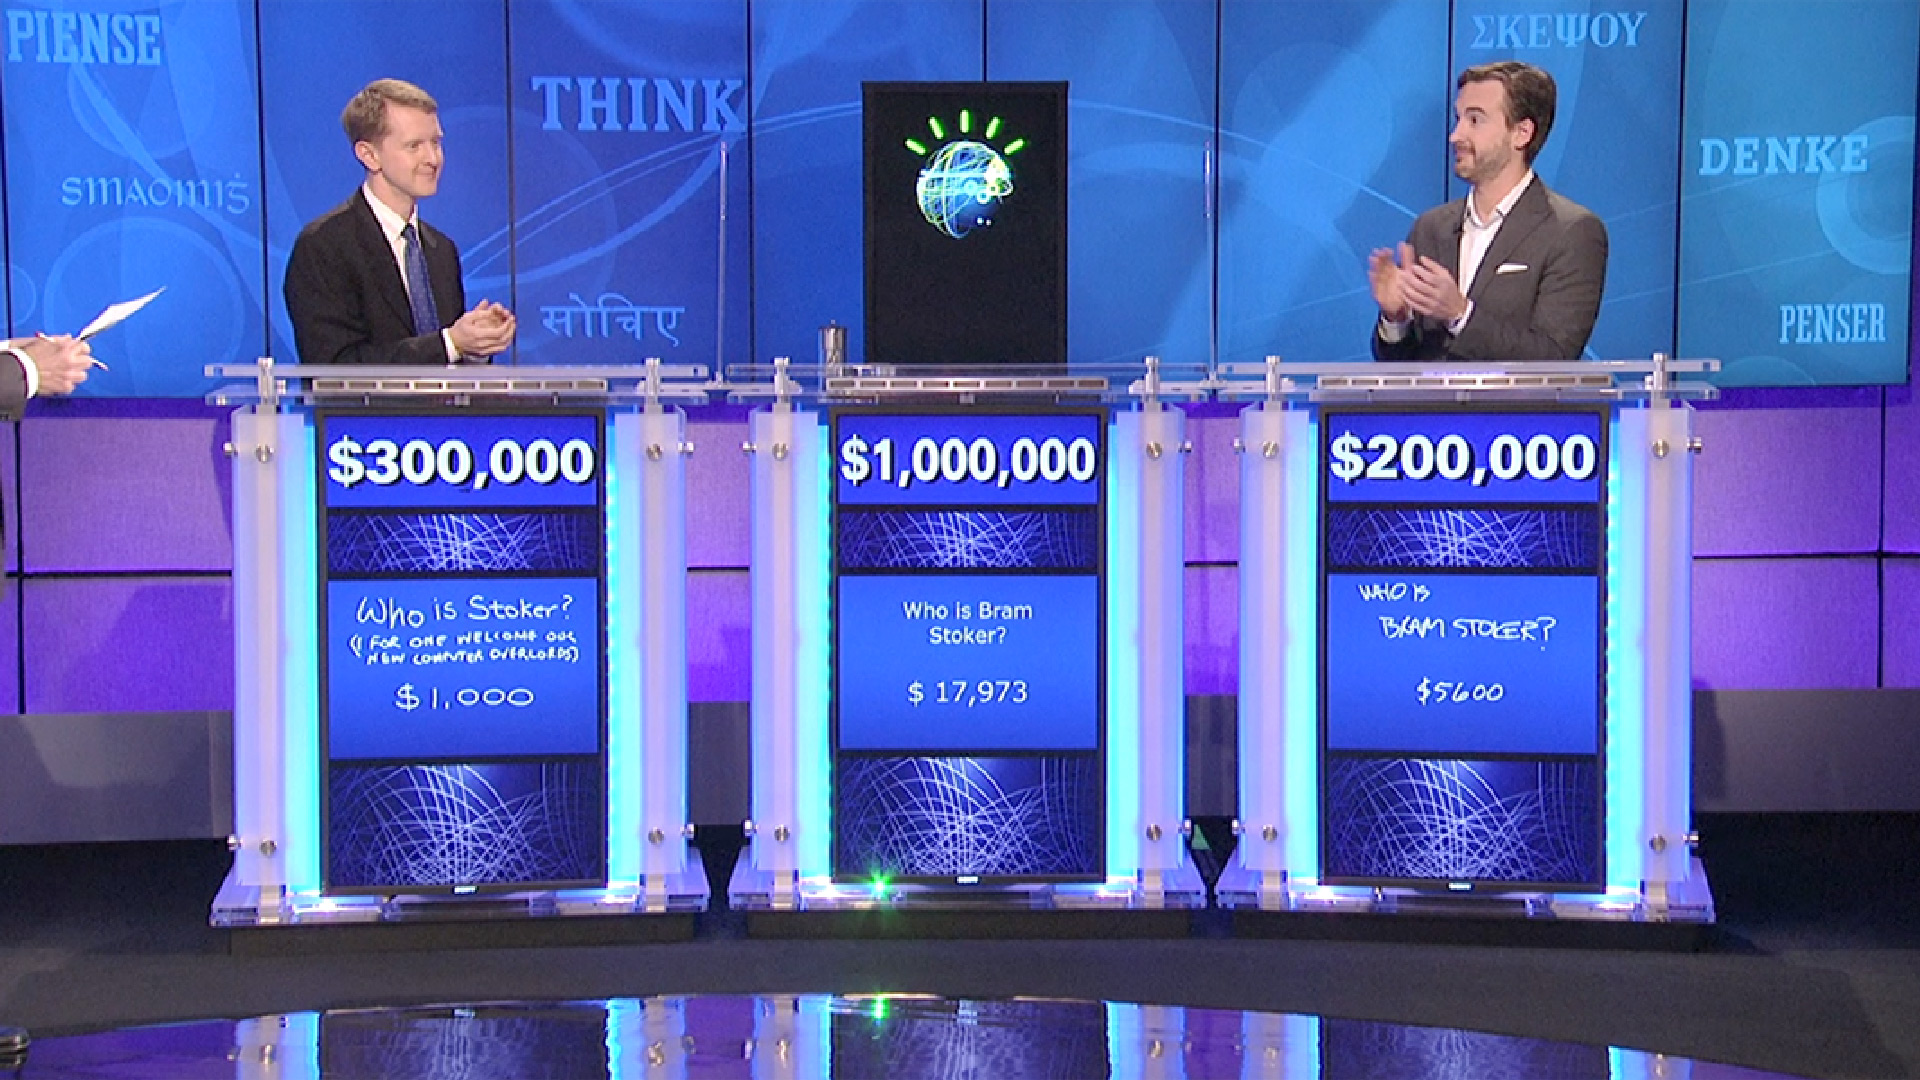
\includegraphics[width=1.0\linewidth]{qb/jeopardy}
                \pause
                \vspace{-8cm}
         \begin{block}{This is {\bf not} Jeopardy}
		\begin{itemize}
                        \item Jeopardy: must decide to answer {\bf once}, after
                          complete question
                        \item Quiz Bowl: decide after each word
		\end{itemize}

	\end{block}

\end{frame}




% TODO add more questions here

\begin{frame}[t]
\frametitle{Sample Question}
	\frametitle{Sample Question}

With Leo Szilard, he invented a doubly-eponymous \only<2->{refrigerator with no moving parts. He did not take interaction with neighbors into account when formulating his theory of} \only<3->{heat capacity, so} \only<4->{Debye adjusted the theory for low temperatures. His} \only<4->{summation convention automatically sums repeated indices in tensor products. His name is attached to the A and B coefficients} \only<5->{for spontaneous and stimulated emission, the subject of one of his multiple groundbreaking 1905 papers. He further developed the model of statistics sent to him by} \only<6->{Bose to describe particles with integer spin. For 10 points, who is this German physicist best known for formulating the} \only<7->{special and general theories of relativity?} \\
\vspace{1cm}
\only<8->{ {\bf Albert \underline{Einstein}}}

\only<9->{
\vspace{-6cm}

\begin{block}{Faster = Smarter}

  \begin{enumerate}
    \item University of Chicago
    \item Colorado School of Mines
    \item Cornell University
    \item UIUC
    \item Brigham Young University
    \item California Institute of Technology
    \item Peking University
    \item Harvey Mudd College
    \item Darmstadt University
    \item University of Colorado
  \end{enumerate}


\end{block}
}

\end{frame}


% \begin{frame}[t]
% 	\frametitle{Sample Question}

%         The Swiss-Italian architect Pietro Antonio Solari
%         \only<2->{built several fortified towers in this city, which
%           often vied for power with its northern rival Tver. A ruler
%           of this city prevailed in the} \only<3->{Great Stand on the
%           Ugra River. A prince from this city was nicknamed for
%           winning a battle on the} \only<4->{Don river. Partly because
%           a ruler of this city married} \only<5->{Sophia Palaiologina,
%           the niece of the last Byzantine Emperor, this city styled
%           itself the} \only<6->{``Third Rome'' after the fall of
%           Constantinople. Another prince of this city stopped paying
%           tribute to the} \only<7->{Mongols in 1476, ending the
%           ``Tatar yoke.''} \only<8->{The Grand Duchy headquartered in
%           this city came to an end in 1547 with the ascension of}
%         \only<9->{ Ivan IV, who made it his capital. For 10 points,
%           name this city where Ivan III renovated the
%           Kremlin,} \only<10->{the capital of Russia.}\\
%         \vspace{.5cm} \only<11->{ {\bf Moscow} (Moskva / Muscovy)}



% \end{frame}





\begin{frame}{}

  \begin{columns}
    \column{.4\linewidth}
        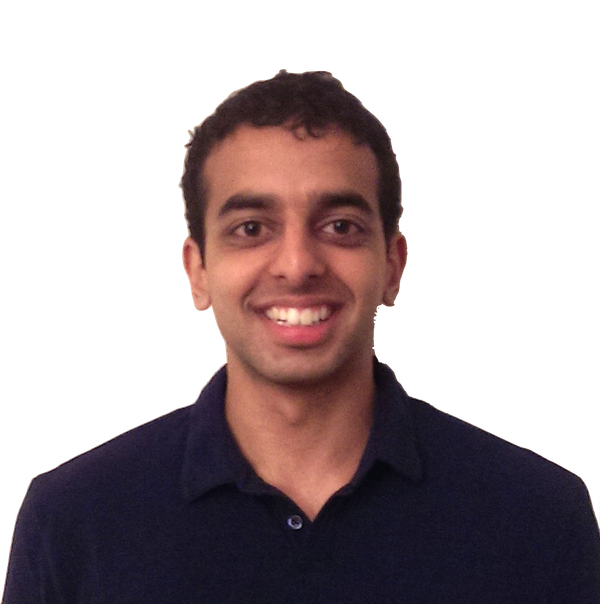
\includegraphics[width=0.7\linewidth]{general_figures/mohit}
    \column{.6\linewidth}
        \begin{block}{ {\bf \href{http://umiacs.umd.edu/~jbg//docs/2014_emnlp_qb_rnn.pdf}{A Neural Network for Factoid Question Answering over Paragraphs}}}
\underline{\href{http://cs.umd.edu/~miyyer/}{Mohit Iyyer}}, {\bf Jordan Boyd-Graber}, Leonardo Claudino, Richard Socher, and Hal {Daum\'{e} III}.  \emph{Empirical Methods in Natural Language Processing}, 2014
        \end{block}

        \begin{block}{ {\bf \href{file:///Users/jbg/public_html/docs/2015_acl_dan.pdf}{Deep Unordered Composition Rivals Syntactic Methods for Text Classification}}}
\underline{\href{http://cs.umd.edu/~miyyer/}{Mohit Iyyer}}, Varun
Manjunatha, {\bf Jordan Boyd-Graber} and Hal {Daum\'{e} III}.  \emph{Empirical Methods in Natural Language Processing}, 2014
        \end{block}

  \end{columns}
\end{frame}


\begin{frame}{Experiment 1}

		\begin{columns}
			\column{.25\linewidth}
				\gfxq{colby_jeo}{1.0}
                                Colby Burnett:
                                \$375,000
			\column{.25\linewidth}
				\gfxq{ben_jeo}{1.0}
                                Ben Ingram:
                                \$427,534
			\column{.25\linewidth}
				\gfxq{alex_jeo}{1.0}
                                Alex Jacobs: \$151,802
			\column{.25\linewidth}
				\gfxq{kristin_jeo}{1.0}
                                Kristin Sausville: \$95,201
		\end{columns}

                \pause


                \begin{center}
                End result: 200-200 tie!
                \end{center}

\end{frame}

\fsi{qb/hsnct1}{}
\fsi{qb/nasat}{Humans 345-145}
\fsi{qb/jennings_handshake}{300-160}
\fsi{qb/hsnct_2017}{Computer 260-215}


\begin{frame}[plain]
\gfxq{seattle_crowd}{.5}
\gfxq{chicago_crowd}{.5}
\end{frame}

\fsi{qb/boring_dot_products}{}

\fsi{simtrans/centaur-chess}{Centaur Chess}


\fsi{qb/augment/screenshot_all}{Interface}

\fsi{qb/augment/screenshot_guesses}{}

\fsi{qb/augment/screenshot_highlight}{{\bf Highlighting}}

\fsi{qb/augment/screenshot_evidence}{}

\begin{frame}{Experts vs. Novices}

 \begin{block}{Experts}
   Trivia experts, familiar with task, enjoy the task
 \end{block}

 \begin{block}{Mechanical Turkers}
   Mechanical Turkers: easily overwhelmed, need the help
 \end{block}

\end{frame}

\fsi{qb/augment/tools_acc}{Evidence helps novices, experts are expert}
% \fsi{qb/augment/tools_buzz}{Highlights help experts}

\begin{frame}{Regression Analysis}
  For each triple (player, question, interpretations), \\
  predict the outcome (correct answer or not) \\
  with logistic regression. Using features:
    \begin{itemize}
        \item \alert<3>{player ID}
        \item \alert<3>{question ID}
        \item buzzing position
        \item enabled interpretations: individual and combinations
    \end{itemize}

    \pause

    \begin{block}{Coefficients tell story!}
      \begin{itemize}
        \item {\bf Big, Positive}: Help
        \item {\bf Big, Negative}: Hurt
        \item {\bf Small}: Neutral
      \end{itemize}
    \end{block}

\end{frame}


\fsi{qb/augment/coefs_0}{Everything helps: Evidence for novies,
  Highlight for experts}
\fsi{qb/augment/coefs_1}{Synergistic effects}
\fsi{qb/augment/coefs_2}{Highlight and evidence help experts most}
\fsi{qb/augment/coefs_3}{For novices, less synergy}


\begin{frame}{}

  \begin{columns}
    \column{.4\linewidth}
    \begin{center}
        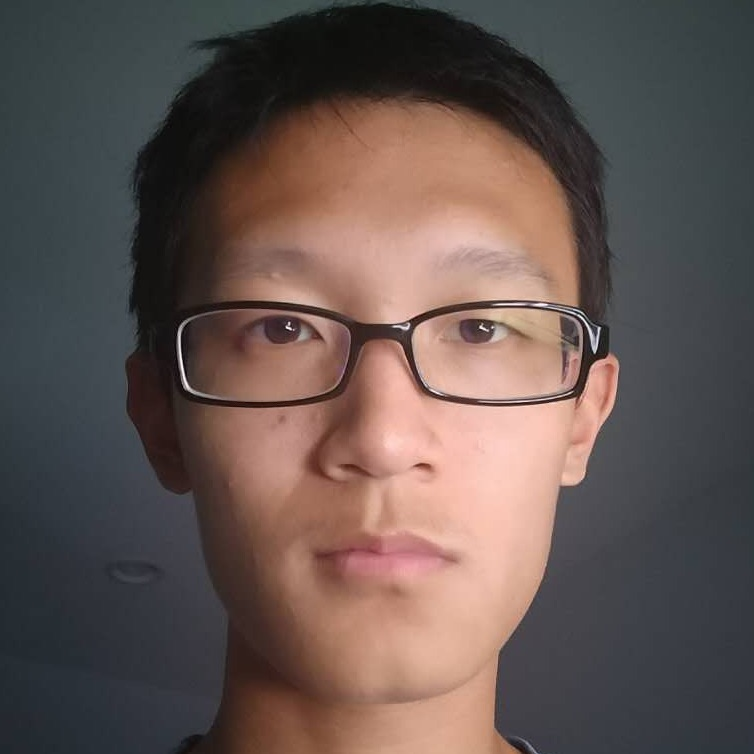
\includegraphics[width=0.8\linewidth]{general_figures/shi}
        \end{center}
    \column{.6\linewidth}
    \begin{block}{\href{http://umiacs.umd.edu/~jbg//docs/2023_emnlp_augment.pdf}{Learning to Explain Selectively}}
      \underline{\href{http://users.umiacs.umd.edu/~shifeng/}{Shi Feng}} and {\bf Jordan Boyd-Graber}.  \emph{Empirical Methods in Natural Language Processing}, 2022
        \end{block}

  \end{columns}
\end{frame}


\begin{frame}{Measuring Interpretability}

  \only<1>{\gfxq{qb_centaur_1}{.9}}
  \only<2>{\gfxq{qb_centaur_2}{.9}}
  \only<3>{\gfxq{qb_centaur_3}{.9}}
  \only<4>{\gfxq{qb_centaur_6}{.9}}


\end{frame}


\begin{frame}{Improvement through Bandit Algorithms}

  \only<1>{\gfxq{rl_centaur_2}{.9}}
  \only<2>{\gfxq{rl_centaur_3}{.9}}
  \only<3>{\gfxq{rl_centaur_4}{.9}}
  \only<4>{\gfxq{rl_centaur_5}{.9}}
  \only<5>{\gfxq{rl_centaur_6}{.9}}

  \only<5->{Bandit actions~\cite{robbins-52}: turn each of the explanations (Guess,
    Highlight, Evidence) on or off.}
\end{frame}

\fsi{qb/augment/bandit_result_none}{Human alone without an AI teammate}
\fsi{qb/augment/bandit_result_ai}{AI alone without a human teammate}
\fsi{qb/augment/bandit_result_dynamic}{Dynamic assistance to human}
\fsi{qb/augment/bandit_result}{Better than showing everything!}

\begin{frame}{Simultaneous Interpretation is Hard!}

  \begin{columns}
    \column{.5\linewidth}
  \begin{itemize}
    \item Exhausting for humans
    \item Computers not trusted
    \item Differential strengths
    \item Same word-by-word characteristic
  \end{itemize}

  \column{.5\linewidth}
 \gfxs{computer-interpreter}{1.0}
 \end{columns}
\end{frame}


\begin{frame}{}
  \begin{columns}
    \column{.2\linewidth}
    \begin{center}
        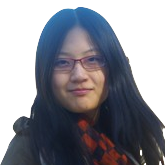
\includegraphics[width=0.8\linewidth]{general_figures/hehe} \\
        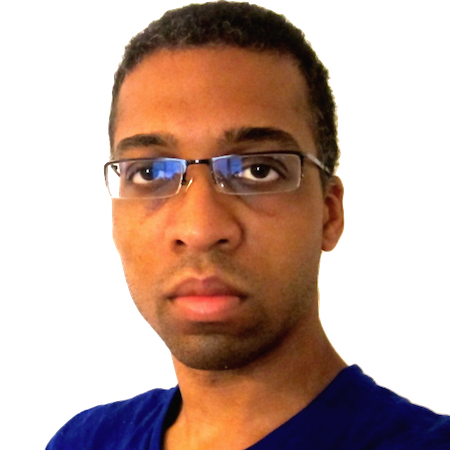
\includegraphics[width=0.8\linewidth]{general_figures/alvin}
        \\
        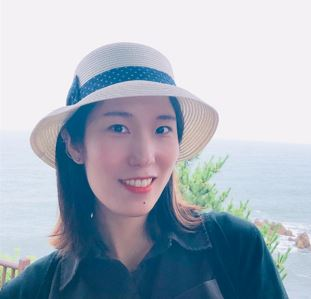
\includegraphics[width=0.8\linewidth]{general_figures/hyojung}
        \end{center}
    \column{.8\linewidth}

        \begin{block}{ {\bf
              \href{http://umiacs.umd.edu/~jbg//docs/2014_emnlp_simtrans.pdf}{Don’t Until the Final Verb Wait: Reinforcement Learning for Simultaneous Machine Translation}}}
          \small
Alvin Grissom II, He He, {\bf Jordan Boyd-Graber}, John Morgan, and Hal {Daum\'{e} III}.  \emph{Empirical Methods in Natural Language Processing}, 2014
        \end{block}

        \begin{block}{ {\bf
              \href{http://umiacs.umd.edu/~jbg/docs/2016_naacl_interpretese.pdf}{Interpretese
                vs. Translationese: The Uniqueness of Human Strategies
                in Simultaneous Interpretation}}}
          \small
He He, {\bf Jordan Boyd-Graber}, and Hal {Daum\'{e} III}.
\emph{North American Association for Computational Linguistics}, 2016
        \end{block}


        \begin{block}{ {\bf
              \href{http://umiacs.umd.edu/~jbg/docs/2022_emnlp_simint.pdf}{SimQA:
                Detecting Simultaneous MT Errors through 
                Word-by-Word Question Answering}}}
          \small
          \href{https://h-j-han.github.io/}{HyoJung Han}, Marine
            Carpuat, {\bf Jordan Boyd-Graber}.  \emph{Empirical Methods in Natural Language Processing}, 2022
          
          \end{block}
  \end{columns}


\end{frame}


\fsi{simtrans/liang_huang}{}
\fsi{simtrans/delay}{}

\begin{frame}{How to Evaluate}

  \begin{columns}
    \column{.5\linewidth}
    \only<1>{
      
\includegraphics[width=1.0\linewidth]{simtrans/polish_jeopardy}}
    \only<2->{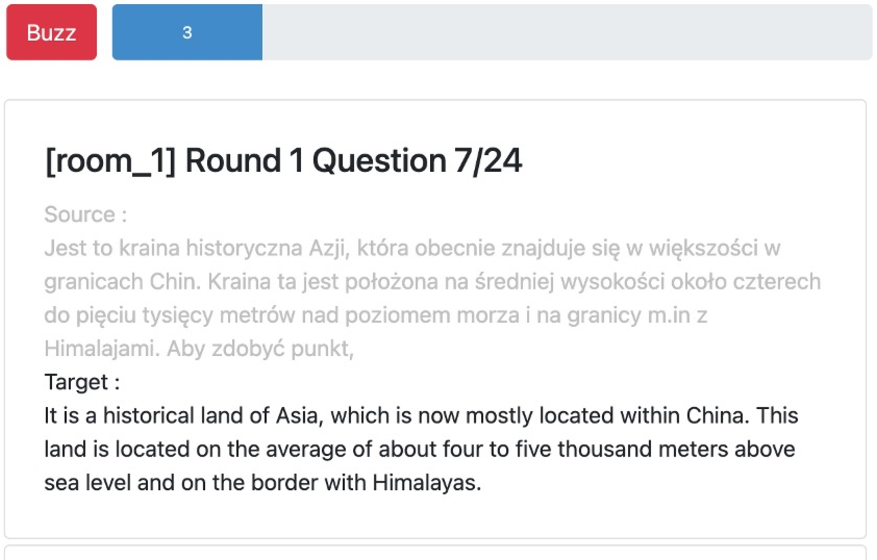
\includegraphics[width=0.8\linewidth]{simtrans/interface}}
    \column{.5\linewidth}
    \begin{itemize}
    \item You're a contestant on a Polish game show
    \item You have access to a simultaneous translation system
    \item Your job is to answer the question before your opponent (as
      quickly as possible)
      \only<3>{\alert<3>{ \item Keep question answerer the same, vary translation}}
    \end{itemize}
  \end{columns}

\end{frame}

\begin{frame}{BLEU results for modern Simultaneous Translation Systems}

  \begin{center}
  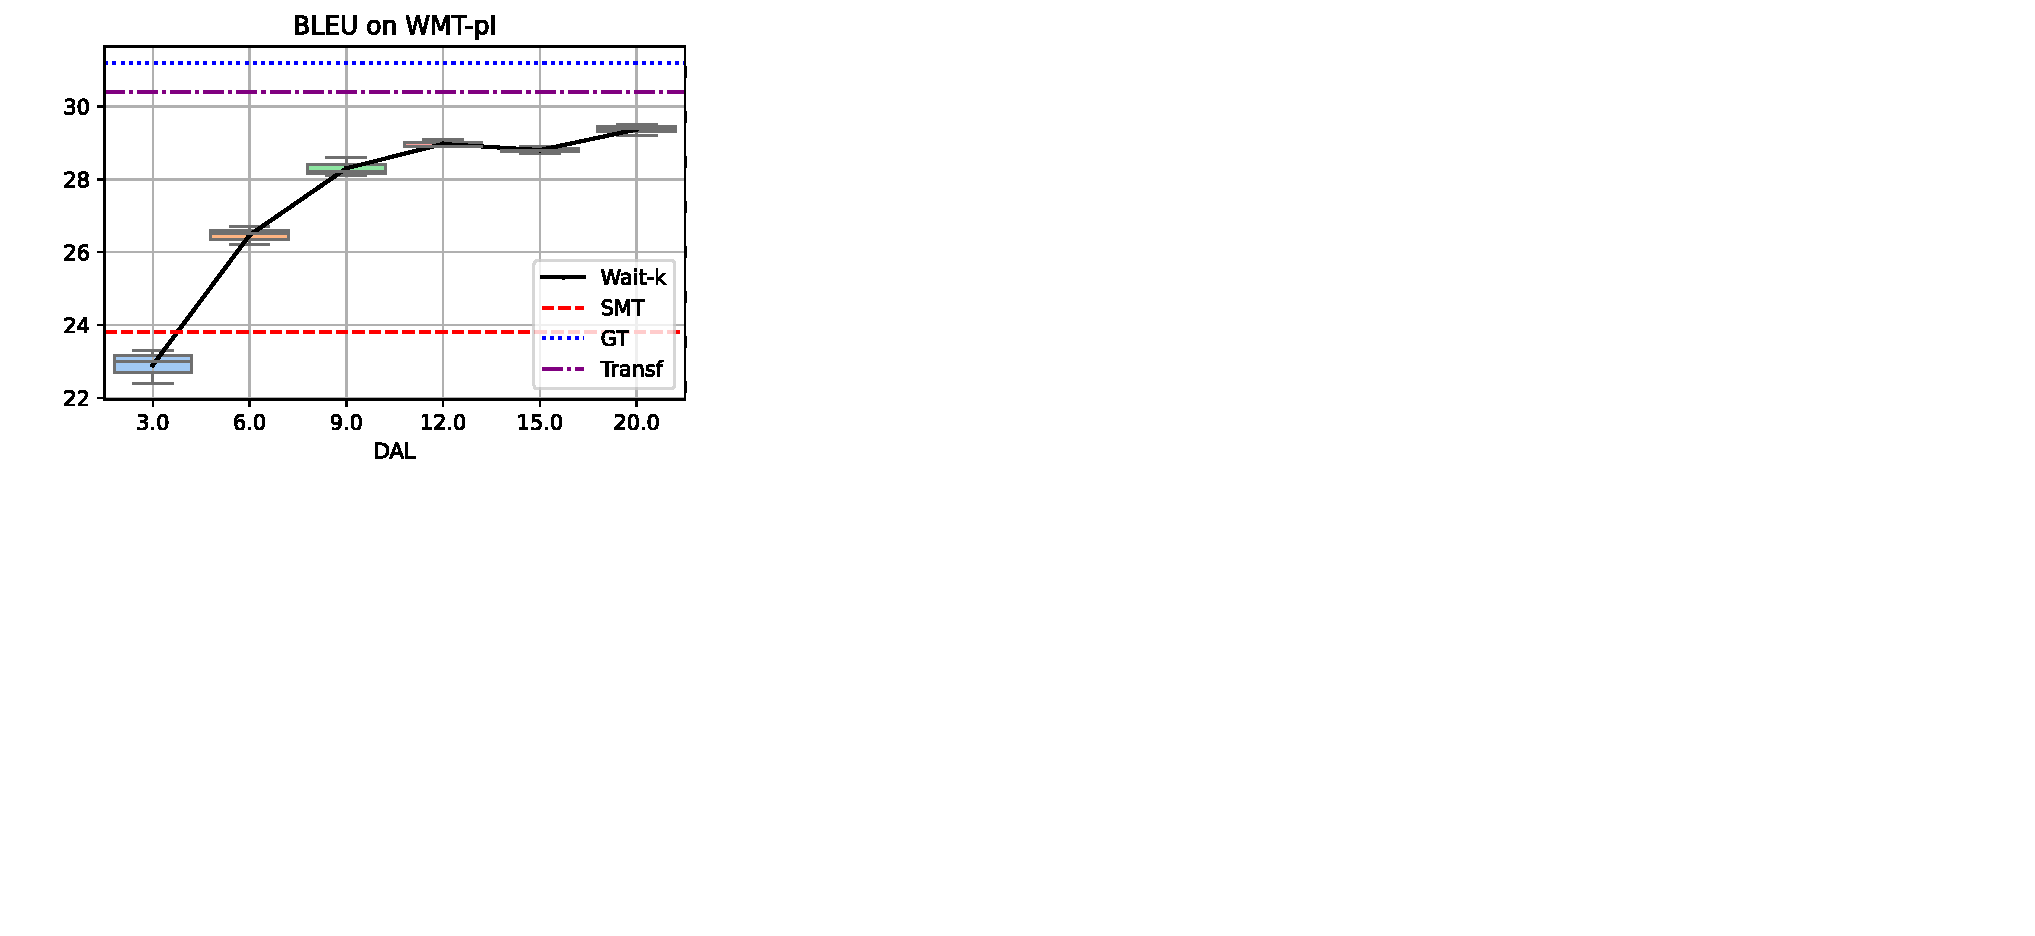
\includegraphics[width=0.9\linewidth]{simtrans/simQA/bleu_simqa}
\end{center}

\end{frame}

\begin{frame}{Downstream QA Results}

  \begin{center}
  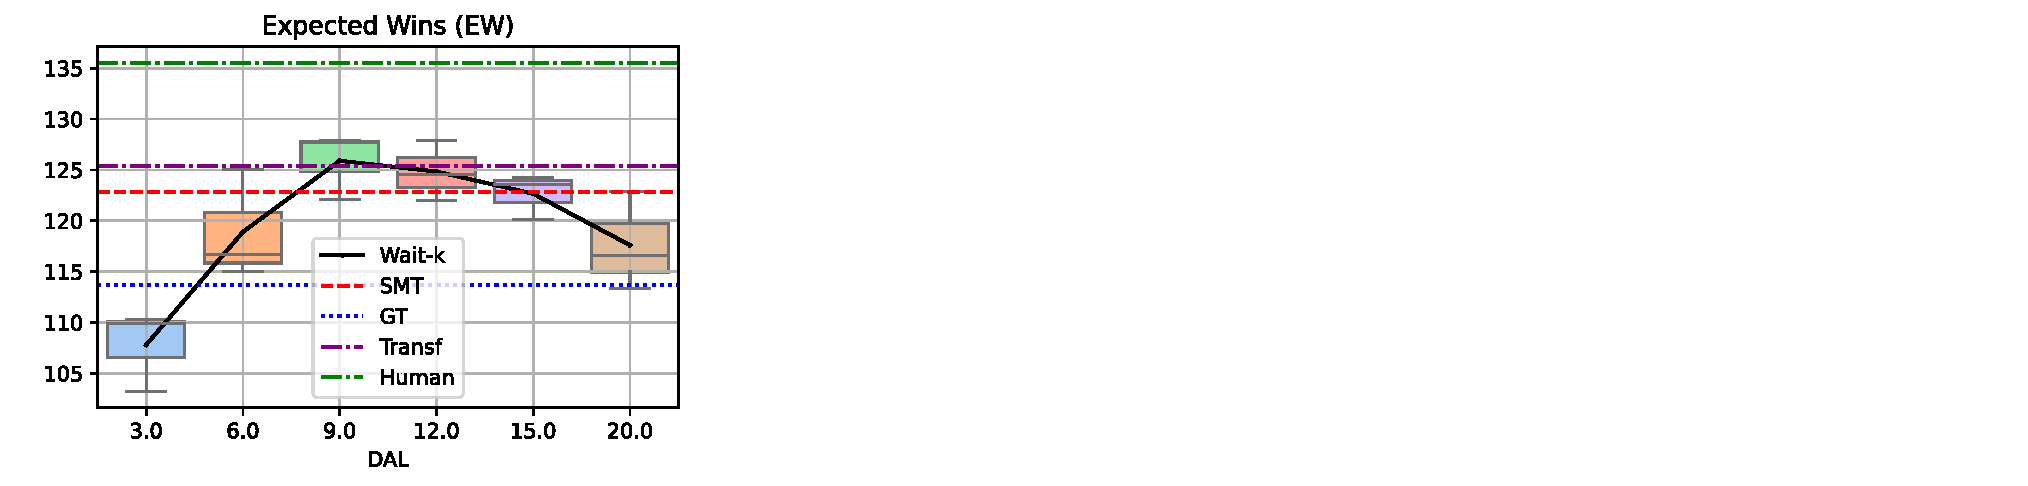
\includegraphics[width=0.8\linewidth]{simtrans/simQA/qametrics_simqa}
\end{center}

\only<2->{Additional benefit: Only need to translate the answer}

\end{frame}


\begin{frame}{Undertranslation}
  \begin{center}
    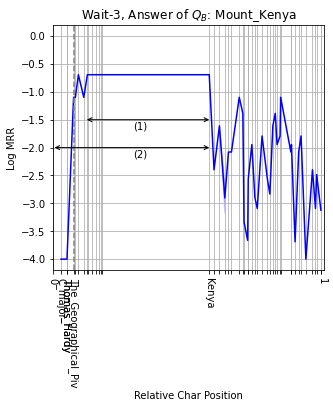
\includegraphics[width=0.4\paperwidth]{simtrans/simQA/ex_undertranslation}
  \end{center}
When the translation doesn't
help\dots
\end{frame}

\begin{frame}{When are Mistakes / Hallucinations Harmful?}


  \begin{center}
    \only<2->{This coordinate determines}
    \only<3->{the double-wall}
    \only<4->{angle between the southern half of the meridian plane
      and the}
    \only<5->{southern}
  \only<1>{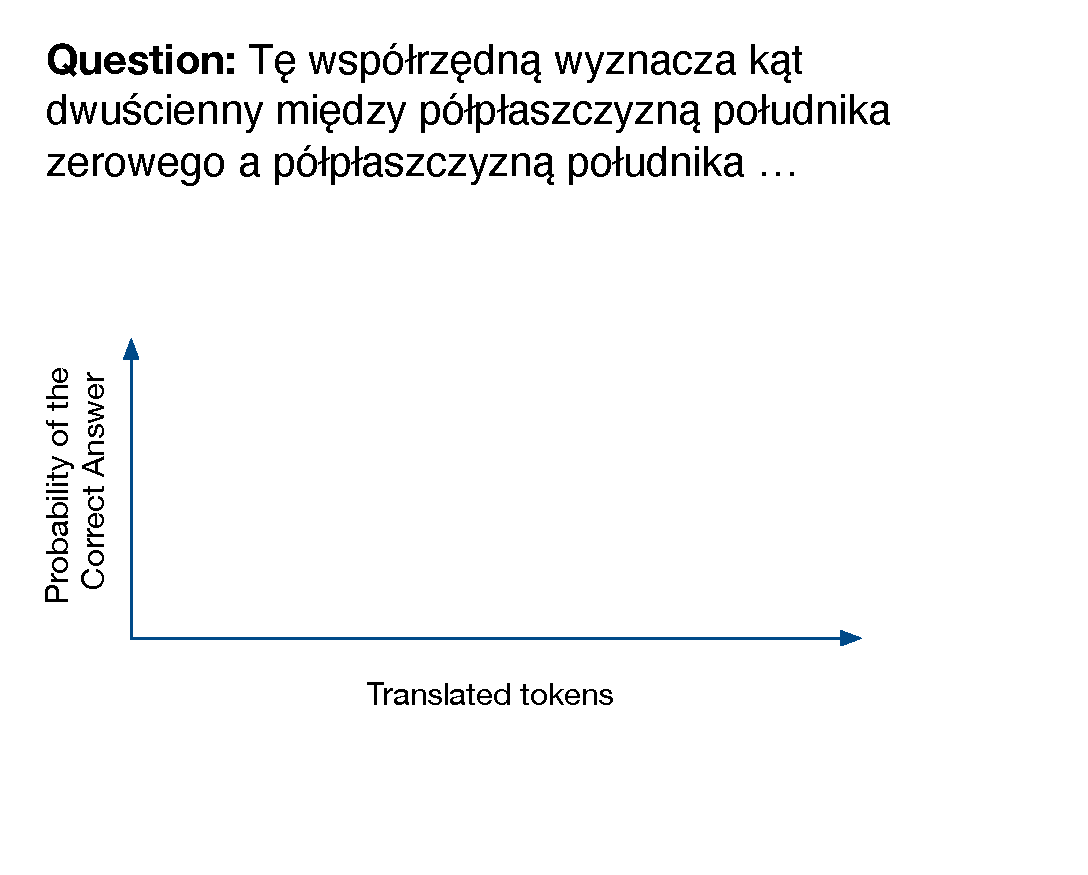
\includegraphics[width=0.5\paperwidth]{simtrans/simQA/hallucination_example_0}}
  \only<2>{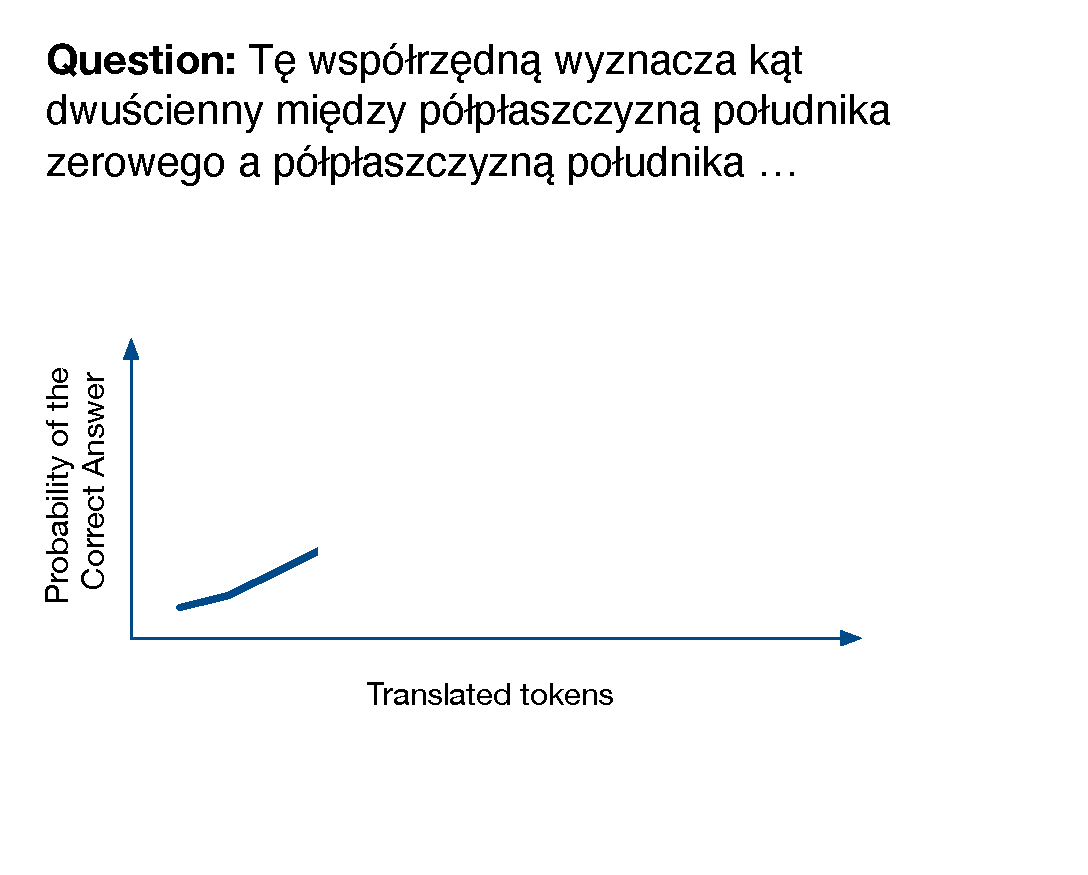
\includegraphics[width=0.5\paperwidth]{simtrans/simQA/hallucination_example_1}}
  \only<3>{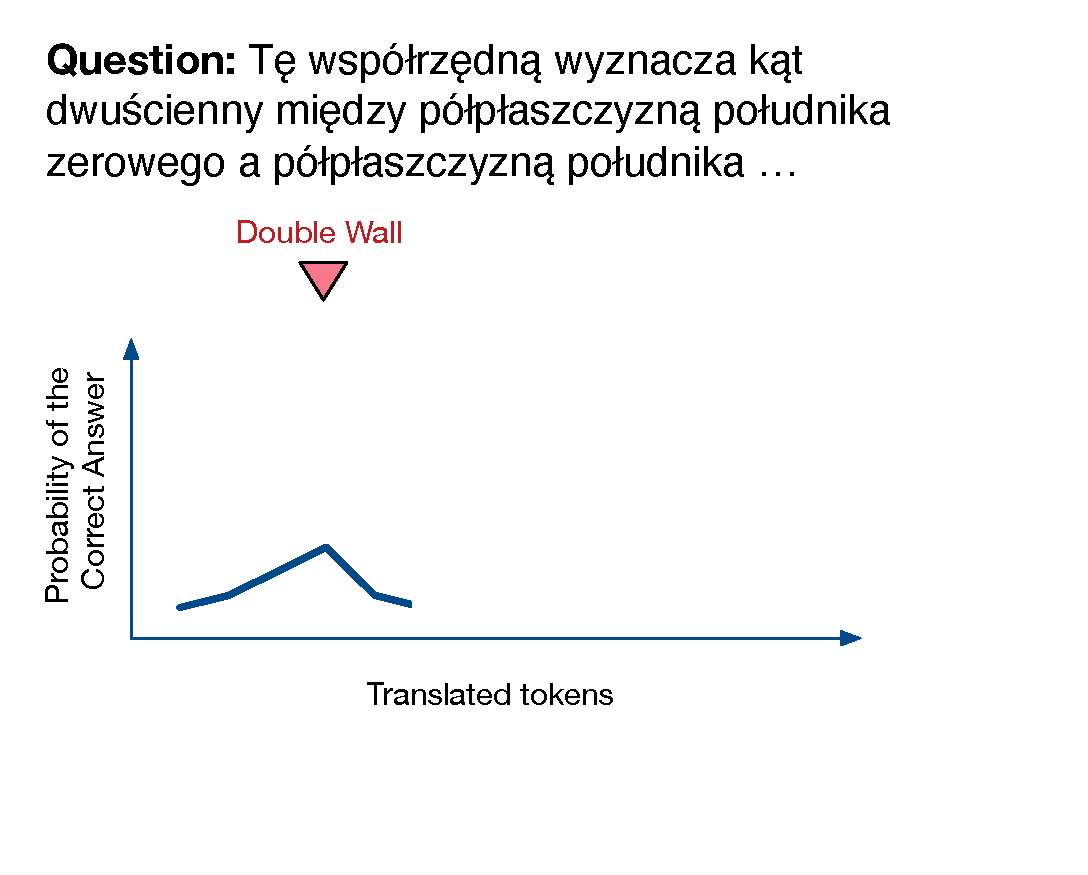
\includegraphics[width=0.5\paperwidth]{simtrans/simQA/hallucination_example_2}}
  \only<4>{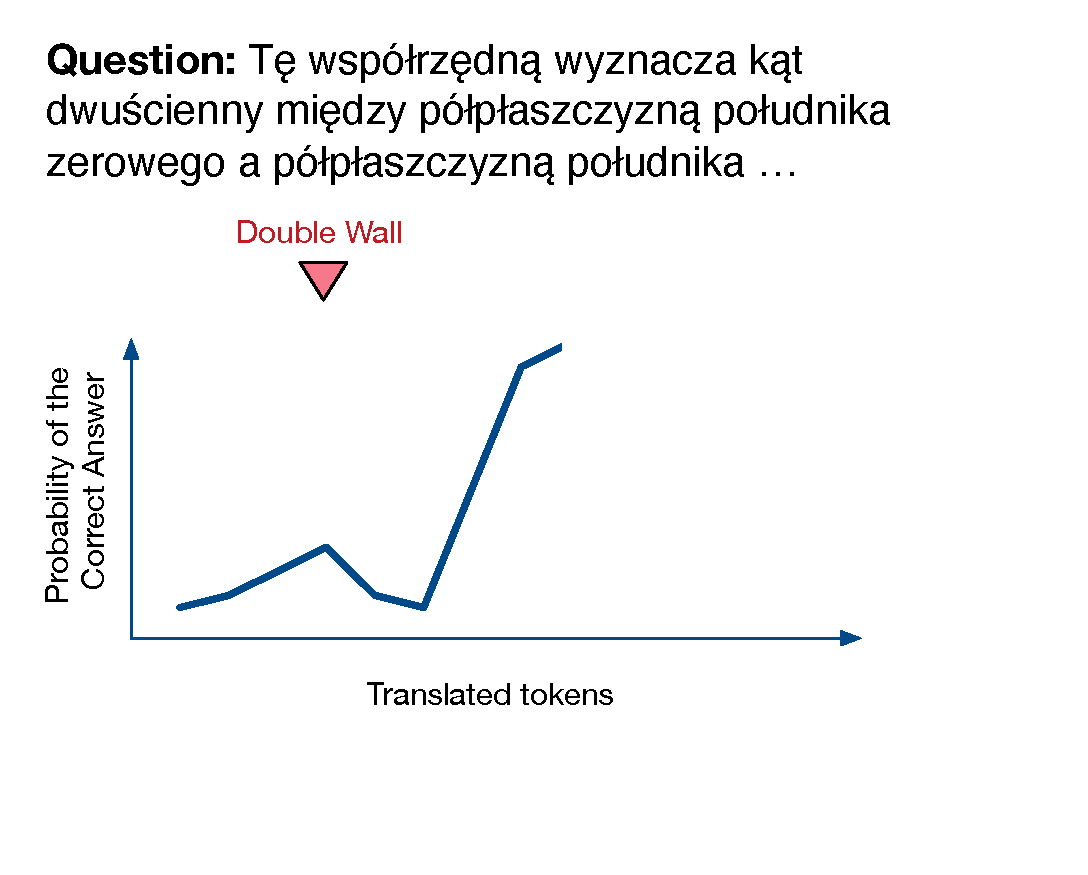
\includegraphics[width=0.5\paperwidth]{simtrans/simQA/hallucination_example_5}}  
  \only<5>{\includegraphics[width=0.5\paperwidth]{simtrans/simQA/hallucination_example_3}}
  \only<6>{\includegraphics[width=0.5\paperwidth]{simtrans/simQA/hallucination_example_4}}
\end{center}
{\bf Guess: } \only<1>{??} \only<2>{IP Address} \only<3>{Spherical
  Coordinate} \only<4>{Longitude} \only<5>{Spherical Coordinate} \only<6>{Longitude}
\end{frame}


\begin{frame}

\makebox[\linewidth]{\includegraphics[width=\paperwidth]{general_figures/blackbox}}
\only<2>{

\vspace{-5cm}
\begin{block}{Takeaways}
  \begin{itemize}
    \item AI should be interpretable
    \item We should measure interpretability
    \item Interpretability should reflect the world we want
  \end{itemize}
\end{block}

}
\end{frame}


\begin{frame}{Future Work}

  \begin{itemize}
  \item Decide as a community what we want
  \item Make it easier for human-driven evaluation
    \item Backpropagate into \emph{generation} of interpretations
    \item Improve data quality with human-in-the-loop adversarial examples
    \item Have better models of individual users (e.g., item response
      theory)
    \item Focus on collaboration
      \begin{itemize}
      \item Triage
      \item Sensemaking
      \item Question answering
        \item Media consumption (fact checking)
      \end{itemize}
  \end{itemize}

\end{frame}

\frame{

	\frametitle{Thanks}

        \begin{block}{Collaborators}
          Hal Daum\'e III (UMD), David Blei (Columbia), Marine Carpuat
          (UMD), Leah Findlater (UW), Kevin Seppi
          (BYU), Eric Ringger (BYU)
        \end{block}

	\begin{columns}

	\column{.75\linewidth}
        \begin{block}{Funders}
        \begin{center}
          \includegraphics[width=0.2\linewidth]{general_figures/nsf}
          \includegraphics[width=0.2\linewidth]{general_figures/darpa}
          \includegraphics[width=0.2\linewidth]{general_figures/arl}
          \includegraphics[width=0.2\linewidth]{general_figures/iarpa}
       \end{center}
        \end{block}

	\column{.3\linewidth}
        \begin{block}{Supporters}
          \includegraphics[width=1.0\linewidth]{general_figures/iac}
        	\gfxq{naqt}{1.0}
        \end{block}

        \end{columns}
}

\frame{
  \frametitle{But wait, there's more!}

  \vspace{-.5cm}

\begin{columns}



  \column{.5\linewidth}

   \begin{block}{Computational Social Science}
     \centering
     \includegraphics[width=0.8\linewidth]{teaparty/figures/framing} \\
     \cite{nguyen-13b,nguyen-15}
   \end{block}


    \begin{block}{Detecting Deception}
    \centering
        \includegraphics[width=0.4\linewidth]{general_figures/diplomacy} \\
        \cite{peskov-20,Eisenschlos-21}
    \end{block}

  \column{.5\linewidth}


    \begin{block}{Multilingual/Multicultural Models}
      \begin{center}
        \includegraphics[width=0.4\linewidth]{general_figures/tonal_translation} \\
      \cite{hu-14,Guo-22}
       \end{center}
    \vspace{-.3cm}
    \end{block}


  \begin{block}{Computational Biology}
     \centering
     \includegraphics[width=0.4\linewidth]{general_figures/protein} \\
     \small
     \cite{nguyen-13b,hu-13:coalescent}
   \end{block}





\end{columns}

}


\frame{

\begin{columns}

\column{.5\linewidth}

\includegraphics[width=.8\linewidth]{general_figures/forough}

\column{.5\linewidth}

\begin{block}{ALTO: Active Learning with Topic Overviews for Speeding Label Induction and Document Labeling}
Forough Poursabzi-Sangdeh, Jordan Boyd-Graber, Leah Findlater, and Kevin Seppi.  Association for Computational Linguistics, 2016.
\end{block}

\end{columns}

}



\fsi{interactive_topic_models/alto_interface}{}
\fsi{interactive_topic_models/alto_interface_highlight}{Direct users
  to document}



\fsi{interactive_topic_models/alto/user_talk_1}{ Active learning if time is short}
\fsi{interactive_topic_models/alto/user_talk_2}{ Better than status quo}
\fsi{interactive_topic_models/alto/user_talk_3}{ Active learning can
  help topic models }
\fsi{interactive_topic_models/alto/user_talk_4}{ Topic models help
  users understand the collection }
\fsi{interactive_topic_models/alto/user_talk_4}{ Moral: machines and
  humans together (if you let them) }


\fsi{qb/viz_first_draft}{Andrea Lin}


\begin{frame}{References}
\bibliographystyle{style/acl}
\tiny
\bibliography{bib/journal-full,bib/jbg,bib/hhe,bib/alvin,teaparty/vietan,bib/hoyle}
\end{frame}



\begin{frame}{RC TRUST}
\begin{center}
  \includegraphics[width=0.7\paperwidth]{job_talks/trust_research_centers}
\end{center}
\small
  \only<2>{
    \begin{columns}
      \column{.6\linewidth}
    \begin{block}{Psychology \& Social Sciences}
      \begin{itemize}
      \item Method: Item Response Theory
      \item Method: Ideal Point Models
        \item Application: Multilingual and Multicultural Models of
          Persuasion and Alliance Building
        \item Collaboration: Bundesverfassungsgericht Entscheidungen
        \end{itemize}
      \end{block}
      \column{.4\linewidth}      
      \end{columns}
  }
  
  \only<3>{
    \begin{columns}
      \column{.1\linewidth}
      \column{.6\linewidth}
      \begin{block}{AI \& ML}
              \begin{itemize}
    \item Method: Reinforcement Learning 
    \item Method: Neural Text Similarity
    \item Application: Training QA Retrieval Mechanisms
    \item Collaboration: Improving Google QA
      \end{itemize}
      \end{block}
      \column{.3\linewidth}      
    \end{columns}
  }


  \only<4>{
    \begin{columns}
      \column{.3\linewidth}
      \column{.6\linewidth}
      \begin{block}{Data Science \& Statistical Learning}
        \begin{itemize}
    \item Method: Bayesian Nonparametrics
    \item Method: Interactive Dirichlet Forest Priors
    \item Application: Sensemaking
    \item Collaboration: Monitoring Local Reseliency
      \end{itemize}
    \end{block}
            \column{.1\linewidth}
  \end{columns}

  }

  \only<5>{
    \begin{columns}
      \column{.4\linewidth}
      \column{.6\linewidth}
    \begin{block}{Cybersecurity and Privacy}
      \begin{itemize}
      \item Method: Adversarial Example Construction
      \item Method: Disinformation Gamefication
      \item Application: Fake News Detection
        \item Collaboration: Climate Fact Checking
      \end{itemize}

    \end{block}
      \end{columns}
  }

  
\end{frame}



\end{document}
